\documentclass[a4paper, 11pt, twoside, openright, title]{book}
\usepackage[T1]{fontenc}
\usepackage[utf8]{inputenc}
\usepackage[linesnumbered,ruled,vlined]{algorithm2e}
\usepackage[english]{babel}
\usepackage{comment}
\usepackage{lscape}

%\usepackage[suftesi]{frontespizio}

% Useful commands
\newcommand{\chapterref}[1]{Chapter \ref{#1}} 
\newcommand{\appendixref}[1]{Appendix \ref{#1}}
\newcommand{\exampleref}[1]{Example \ref{#1}} 
\newcommand{\sectionref}[1]{Section \ref{#1}} 
\newcommand{\figureref}[1]{Figure \ref{#1}} 
\newcommand{\tableref}[1]{Table \ref{#1}} 
\newcommand{\grassetto}[1]{\textbf{#1}} 
\newcommand{\corsivo}[1]{\textit{#1}}

%renew
\renewcommand{\thealgocf}{}


% Colours definitions
\usepackage[usenames,dvipsnames, table]{xcolor}
\colorlet{myred}{red!90}
\colorlet{mygreen}{Green!90}
\definecolor{mygray}{rgb}{0.5,0.5,0.5}
\definecolor{mymauve}{rgb}{0.58,0,0.82}

% Tables
\usepackage{multirow,bigdelim}

% Definitions/Theorems/Examples
\usepackage{amsthm}
\usepackage{amsfonts}
\usepackage{amsmath}
\usepackage{braket}
\theoremstyle{definition}
\newtheorem{definition}{Definition}[chapter]

% Chapter style
\usepackage{titlesec}
\newcommand{\setChapters}[1]{
\titleformat{\chapter}
  [display]{\Large\bfseries} 
  {\hfill #1 \thechapter}
  {0.05ex} {\vspace{-1.2ex}
   \rule{\textwidth}{0.4pt}
   \vspace{-2.4ex}\\}[]}

% Header style
\usepackage{fancyhdr}
\pagestyle{fancy}
\renewcommand{\headrulewidth}{0.4pt}
\renewcommand{\chaptermark}[1]%
{\markboth{\textbf{\chaptername\ \thechapter.\ #1}}{}}
\renewcommand{\sectionmark}[1]%
{\markright{\textbf{\thesection.\ #1}}}
\fancyhf{}
\fancyhead[LO]{\rightmark}
\fancyhead[RE]{\leftmark}
\fancyhead[LE,RO]{\textbf\thepage}

\fancypagestyle{plain}{%
\renewcommand{\headrulewidth}{0pt}
\fancyhf{}}

% Tikz
\usepackage{tikz}
\tikzstyle{bitvector} = [ thick,
  font=\scriptsize, align = center,
  rectangle, rounded corners]

% Listings
\usepackage{listings}


\lstset{
  % Margins
  xleftmargin=0.5cm,
  xrightmargin=0cm,
  framexleftmargin=0.5cm,
  framexrightmargin=0cm,
  % Style
  basicstyle=\ttfamily\footnotesize,  
  keywordstyle=\bfseries,
  commentstyle=\color{black},
  backgroundcolor=\color{white},   % choose the background color; you must add \usepackage{color} or \usepackage{xcolor}
  basicstyle=\footnotesize,        % the size of the fonts that are used for the code
  breakatwhitespace=false,         % sets if automatic breaks should only happen at whitespace
  breaklines=true,                 % sets automatic line breaking
  captionpos=b,                    % sets the caption-position to bottom
  %commentstyle=\color{mygreen},    % comment style
  deletekeywords={...},            % if you want to delete keywords from the given language
  escapeinside={\%*}{*)},          % if you want to add LaTeX within your code
  extendedchars=true,              % lets you use non-ASCII characters; for 8-bits encodings only, does not work with UTF-8
  %frame=single,	                   % adds a frame around the code
  keepspaces=true,                 % keeps spaces in text, useful for keeping indentation of code (possibly needs columns=flexible)
  keywordstyle=\color{black},       % keyword style
  language=C++,                    % the language of the code
  otherkeywords={*,...},           % if you want to add more keywords to the set
  numbers=left,                    % where to put the line-numbers; possible values are (none, left, right)
  numbersep=5pt,                   % how far the line-numbers are from the code
  numberstyle=\tiny\color{black}, % the style that is used for the line-numbers
  rulecolor=\color{black},         % if not set, the frame-color may be changed on line-breaks within not-black text (e.g. comments (green here))
  showspaces=false,                % show spaces everywhere adding particular underscores; it overrides 'showstringspaces'
  showstringspaces=false,          % underline spaces within strings only
  showtabs=false,                  % show tabs within strings adding particular underscores
  stepnumber=1,                    % the step between two line-numbers. If it's 1, each line will be numbered
  stringstyle=\color{black},       % string literal style
  tabsize=2,                   % sets default tabsize to 2 spaces
  title=\lstname        
}

%\newcommand{\lstcinputlisting}[1]{\lstinputlisting[style=CPP]{#1}}

% Bibliography
\usepackage[backend=bibtex, defernumbers=false, maxnames=10]{biblatex}
\usepackage{filecontents}
\bibliography{bibliography}
%\defbibfilter{papers}{type=article or type=inproceedings}
%\defbibfilter{books}{type=book}
%\defbibfilter{others}{not type=article and not type=inproceedings and not type=book}

\usepackage{fixltx2e}
\newcommand{\apsl}{A\textsubscript{P}SL}

\usepackage{enumitem}

% Referencesfa
\usepackage{hyperref}
\hypersetup{hidelinks}

% AcronymsR
\usepackage{acronym}
\usepackage{adjustbox}
\usepackage{pdfpages}

\setlength{\headheight}{14pt} 
%\setcounter{secnumdepth}{3} % seting level of numbering (default for "report" is 3). With ''-1'' you have non number also for chapters
%\setcounter{tocdepth}{3}

\begin{document}

% ---------------------------------------------------------------
% Frontmatter 
% ---------------------------------------------------------------
\frontmatter

% First page
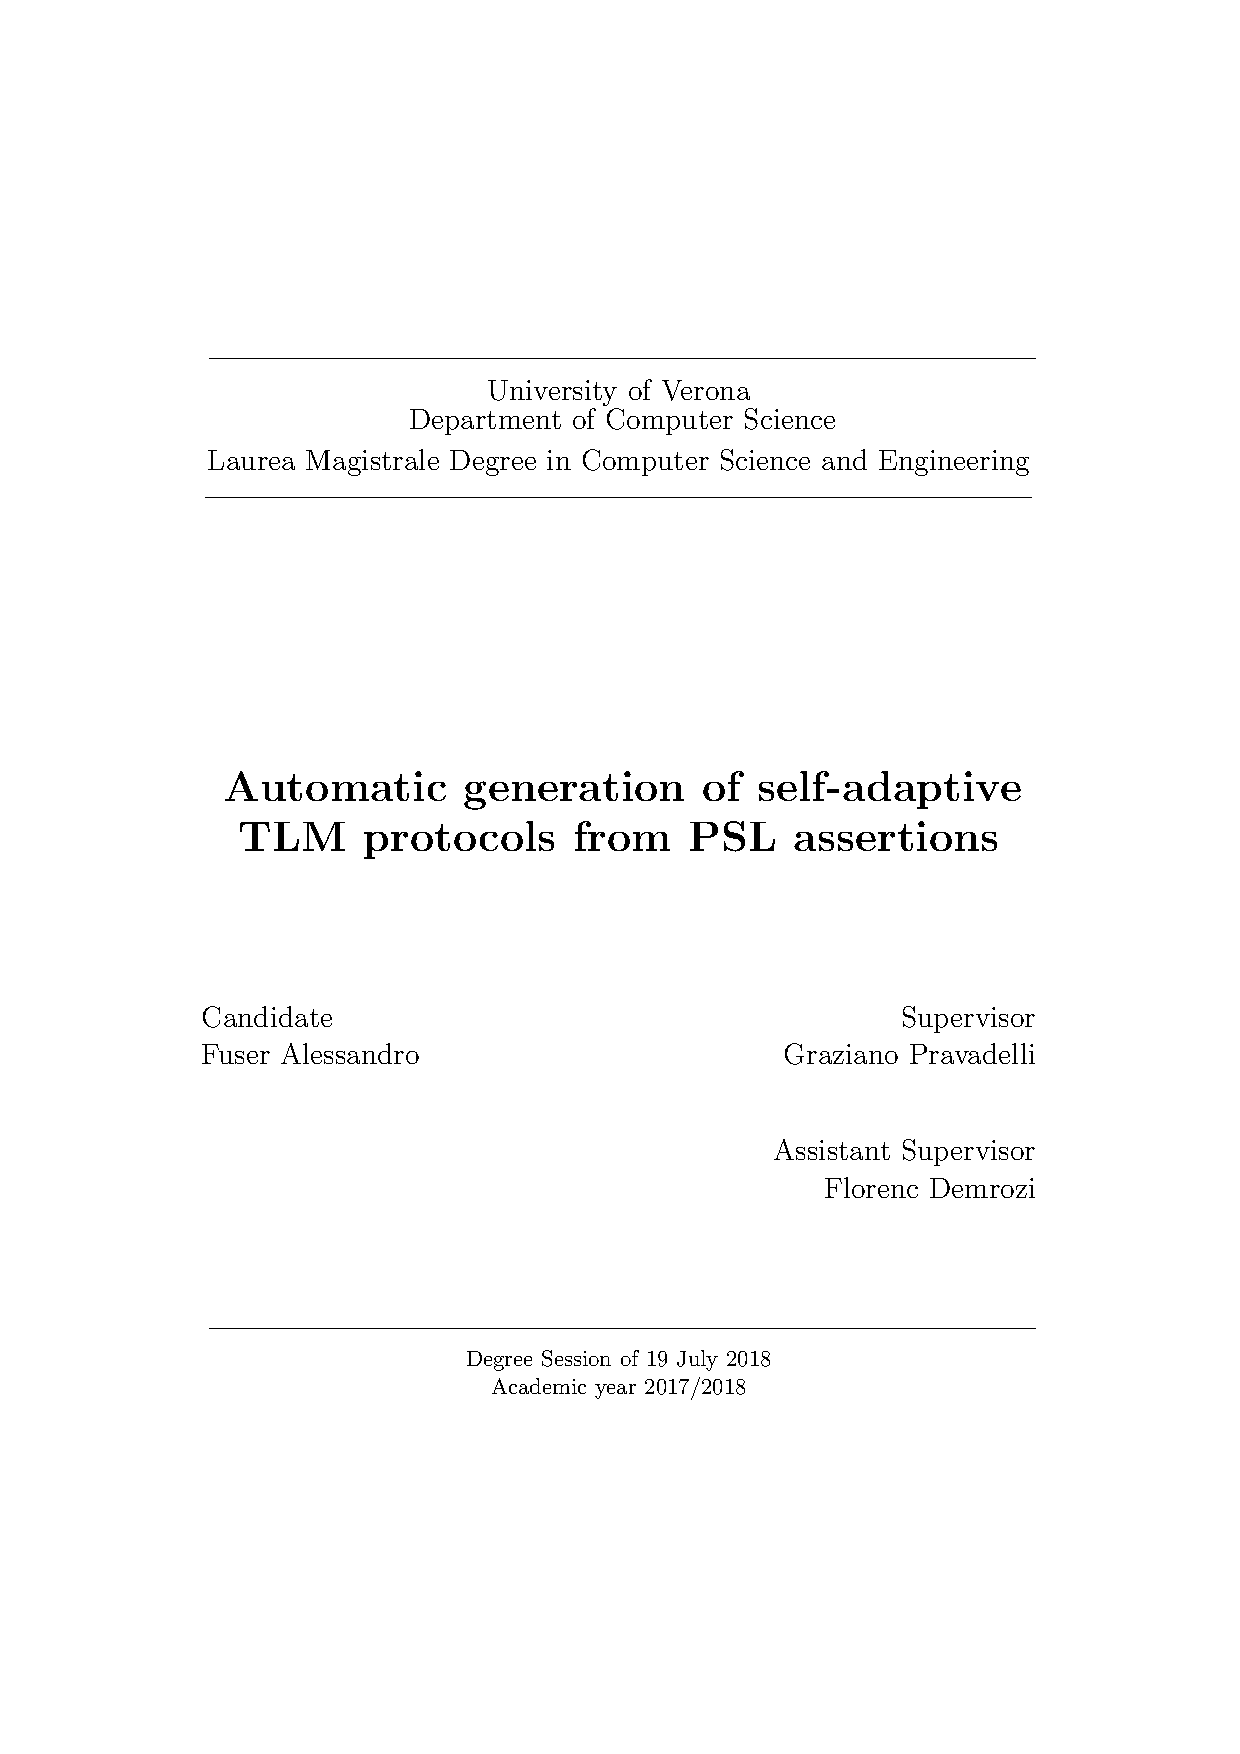
\includepdf{titlepage/titlepage.pdf}
\clearpage\thispagestyle{empty}
% Dedication
% Abstract
\setChapters{Chapter}
\fancyhead[LO, RE]{\textbf{Contents}}
% !TEX root = ../main.tex

\cleardoublepage
\thispagestyle{empty}

\leavevmode \\[0.86cm]
\begin{center}
\rule{\textwidth}{.4pt} \\
\end{center}
{\LARGE\textbf{Abstract}}
\vspace{1cm}

Freezing of gait (FOG) is defined as a brief, episodic absence or marked reduction of forward progression of the feet despite the intention to walk. It is one of the most debilitating motor symptoms in patients with Parkinson's disease (PD) as it may lead to falls and a loss of independence. The pathophysiology of FOG seems to differ from the cardinal features of PD and is still largely unknown. In this paper, we focus on demonstrate the existence of some movements that could lead to FoG and we include this movements in a new class that we call preFoG. We also have conducted an exhaustive study on the right choose of the interval and overlap to better divide our classes, noFoG, preFoG and FoG. We have made a first data classification approach using the preFoG class. At the same time, we conducted a study using clustering algorithms in order to try to replace the doctor in the first phase of data label generation. We have concluded that the best data division interval is 2 seconds window and 1 second overlap. For the classification we arrived at an accuracy of 90\% using data from more patients, while for the clustering phase at an accuracy of 70\%.

\clearpage
\thispagestyle{empty}
% Acknowledgements
% !TEX root = ../main.tex
\chapter{Ringraziamenti}\label{acknowledgements}

% Table of contents

\fancyhead[LO, RE]{\textbf{Contents}}
\tableofcontents
%\listoftables
\listoffigures
% ---------------------------------------------------------------
% Mainmatter 
% ---------------------------------------------------------------
\mainmatter

% Chapters
\fancyhead[LO]{\rightmark}
\fancyhead[RE]{\leftmark}
% !TEX root = ../main.tex

% ---------------------------------------------------------------
% Introdaction
% ---------------------------------------------------------------


\chapter{Introduzione}\label{cap1:Introduzione}

% ---------------------------------------------------------------
% Introdaction
% -Motivation
% ---------------------------------------------------------------
La Malattia di Parkinson è una patologia neurodegenerativa che coinvolge in maniera elettiva la capacità di programmare ed eseguire il movimento, senza risparmiare altri aspetti dell’individuo come la sfera cognitiva e comportamentale. Questi aspetti, unitamente al decorso cronico e progressivo della malattia, determinano una compromissione delle attività di vita quotidiana e delle relazioni interpersonali.

Tra i sintomi della malattia di Parkinson, il Freezing of Gait (FOG) può sicuramente essere considerato uno dei più debilitanti. Il Freezing nella malattia di Parkinson, detto anche congelamento o semplicemente blocco motorio, è un’improvvisa, temporanea e involontaria incapacità di iniziare un movimento. È un disturbo che insorge nel corso dell’evoluzione della malattia di cui costituisce un sintomo indipendente e generalmente resistente al trattamento con levodopa. Tale fenomeno si può verificare in ogni momento e i pazienti che lo sperimentano affermano che: \textit{«è come se i piedi rimanessero, per qualche istante, incollati al suolo con la conseguente impossibilità di eseguire il passo successivo»}. In realtà, il Freezing si può verificare anche durante azioni differenti dal cammino come ad esempio l’alzarsi da una sedia o il raccogliere un oggetto. Alcune persone sono più predisposte di altre a subire episodi di congelamento. Tali episodi, si possono verificare sia quando il soggetto è in astinenza da farmaci dopaminergici, in questo caso si parla di “Freezing off”, sia quando il soggetto sta assumendo i farmaci, “Freezing on”. \\

% ---------------------------------------------------------------
% Introdaction
% -Motivation
% -Methodology
% -Thesis Contribution
% ---------------------------------------------------------------
\section{Contributo della Tesi}\label{cap1:Contributo della Tesi}
In questa lavoro di tesi, si è cercati di sviluppare una metodologia di identificazione degli episodi di FoG e preFoG, ossia una fase transitoria tra un'attività normale ed un episodio di Freezing. Questo è un problema molto debilitante per i malati di Parkinson che, allo studio attuale, non ha una soluzione efficace dal punto di vista medico e di cui non si conoscono a fondo le cause.\\
Per sviluppare tale metodologia, è stato utilizzato un dataset in cui sono presenti 10 pazienti, tutti affetti dal morbo di Parkinson, ed 8 di loro presentano episodi di FoG. I contesti di FoG sono stati identificati dal dottore tramite l'utilizzo di videoregistrazioni ed i dati sono stati raccolti attraverso 3 accelerometri, posizionati sulla caviglia, sul ginocchio e sulla zona lombare del paziente.\\
Il primo passo è stato quello di verificare che può esistere una distinzione tra le 3 classi del nostro dataset, ossia attività normale, preFoG e FoG tramite l'utilizzo di un Linear Discriminant Analysis (LDA). Una volta verificato, e' stato condotto uno studio sugli intervalli con cui dividere i dati del dataset, cioè quanto deve essere grande la finestra temporale su cui calcolo le feature dai dati grezzi e quanta sovrapposizione è opportuno avere. Questo studio è stato condotto sia usando LDA che usando un approccio di clustering, che permette di etichettare i dati senza sapere a quale classe appartengano, al fine di cercare di sostituire il dottore nella prima fase di test. Infine, si accenna ad un primo approccio di classificazione per la previsione di classi su nuovi dati.

% ---------------------------------------------------------------
% Introdaction
% -Motivation
% -Methodology
% -Thesis Contribution
% -Outline
% ---------------------------------------------------------------

Il resto della tesi è organizzata nel modo seguente: nel \textbf{\chapterref{chap2:related}} si presentano i risultati dei principali lavori svolti sul FoG; nel \textbf{\chapterref{chap3:background}} si presentano a livello teorico le problematiche del FoG e gli strumenti su cui si basa il lavoro svolto; nel \textbf{\chapterref{chap4:Goals}} si presenta qual'è l'obiettivo finale del lavoro che viene svolto; nel \textbf{\chapterref{chap5:Automatic}} si presenta il lavoro svolto; nel \textbf{\chapterref{chap9:Concl}} si riassumo i risultati ottenuti e si presentano possibili miglioramenti al lavoro svolto.
 
% !TEX root = ../main.tex

% ---------------------------------------------------------------
% RELATED WORKS
% ---------------------------------------------------------------

\chapter{Letteratura}\label{chap2:related}
Il problema del FOG è stato analizzato tramite una grande varietà di sistemi e sensori. Alcuni di questi, però, non sono utilizzabili durante la vita quotidiana dei pazienti poiché posso essere disponibili solo in ambienti di laboratorio. Esempi di questi sistemi sono le piattaforme di pressione\cite{38}, le quali sono non portatili, l'elettromiografia (EMG)\cite{25}, l'elettroencefalogramma (EEG)\cite{42} o la conduttanza della pelle\cite{43}, il quale comporta il pizzamento di elettrodi sulla pelle in aggiunta ad sistema di rilevamento per raccogliere i dati.
Altri sistemi invasivi sono i goniometri a ginocchio\cite{23} o sistemi che fanno uso di camere e video, i quali hanno una bassa tolleranza del paziente in un'ambiente che non sia di laboratorio\cite{23,39,44}. Quindi, dato che il monitoraggio del PD dovrebbe essere deambulatorio e  durare diverse ore al fine di ricavare utili informazioni cliniche\cite{34,45}, la maggior parte dei lavori si è basata su sistemi non invasivi come i dispositivi indossabili basati su circuiti microelettromeccanici (MEMS). \newline
Nel 2003, Han et al. hanno usato MEMS basati su sistemi inerziali, come gli accelerometri, per esplorare le caratteristiche collegate agli episodi di FoG. Hanno trovato che la frequenza di risposta nei pazienti che indossavano gli accelerometri nella caviglia era intorno ai 6-8 Hz\cite{19}. Nel 2008, Moore et al. hanno proposto una metodologia per identificare FoG con un'accelerometro posizionato nella caviglia nella quale hanno descritto il Freezing Index (FI), ossia il quoziente del rapporto della densità spettrale di potenza (PSD) tra 3 ed 8 Hz, chiamata Freezing Band (FB), con la PSD tra 0.5 e 3 Hz, denominata Walking Band (WB)\cite{21}. Quando il FI supera una certa soglia (Freezing Threshold (FTH)), si considera che si sia verificato un episodio di FoG. A causa della presenza dei falsi positivi (FP) quando il paziente è a riposo, Bachlin et al. hanno introdotto il concetto di Power Index (PI), definito come la somma della WB e FB, il quale viene comparato con la Power Threshold (PTH) al fine di stabilire se c'era una quantità rilevante di movimento nel momento in cui il FI era alto, ossia oltre la soglia\cite{21}. PI indica la quantità di movimento, perciò situazioni nelle quali il paziente non si stesse movendo volontariamente sono state eliminate. In quest'ultima versione dell'algoritmo, quindi, un espisodio di FoG è occorso se FI>FTH e PI>PTH. Questo metodo è il più avanzato nella detenzione di FoG dato il suo scarso costo computazionale e le sue buone performance\cite{22}. \newline
L'algoritmo MBFA è stato ampiamente utilizzato nell'analisi del FoG, anche se di solito in condizioni di laboratorio e molto spesso con pochi pazienti. Jovanov et al. hanno implementato un algoritmo real time, anche se un solo volontario è stato usato per testare l'algoritmo. Inoltre, nessun risultato su sensitività e specificità è stato riportato\cite{22}. Zabaleta et al. hanno analizzato il FoG per mezzo di accelerometri a tre assi e giroscopi a due assi in differenti locazioni degli arti inferiori. La caratteristica principale ad essere stata analizzata è il FI in congiunzione con i cambiamenti della densità spettrale di potenza. Sono stati capaci di identificare correttamente l'82.7\% delgi episodi di FoG con i sensori inerziali posizionati su entrambe le caviglie, anche se in soli 2 pazienti\cite{24}.  \newline
Negli anni più recenti, Niazmand et al. (2011) hanno presentato il Mimed-Pants\cite{26}, pantaloni da jogging lavabili con 5 accelerometri integrati. Hanno usato MBFA per identificare FoG, ottenendo un 88.3\% in sensitività e 85.3\% in specificità con 6 pazienti in brevi e controllati test focalizzati nell'indurre FoG senza tenere conto dei FP. Nel 2012, Zhao et al.\cite{46} hanno sviluppato un algoritmo embedded basato sull'approccio MBFA all'interno del sistea Mimed-Pants ottenendo un 81\% in sensitività con 8 pazienti usando dei test simili ai precedenti. Più recentemente, Mazilu et al. hanno poposto un nuovo algoritmo online usando 3 accelerometri ed comparando diversi classificatori di machine learning che sfruttavano le caratteristiche del MBFA, aggiungendone di nuovo, in 10 pazienti\cite{48}. I risultati ottenuti sono stati migliori del 95\% per specificità e sensitività con differenti classificatori. Questi test, però, sono stati condotti in situazioni di controllo ed, inoltre, la metodologia di validazione sovrastimava le prestazioni delle misure poichè i classificatori erano allenati, iterativamente, con tutte le finestre del segnale disponibili da un paziente escludendone una, la quale veniva usata per ottenere le prestazioni citate. Inoltre, le sequenze di allenamento e di test erano molto simili, il che è molto diverso da normali situazioni. Quindi, ci si aspetta che le riportate specificità e sensitività calino drasticamente in situazioni non controllate. \newline
Nel 2013, Moore et al. hanno pubblicato il più recente lavoro focalizzato sul MBA. In questo, hanno confrontato differenti configurazioni applicando lo stesso algoritmo in 25 pazienti, dei quali 20 hanno avuto episodi di FoG. Diverse finestre di segnale, posizionamento dei sensori e valori per PTH e FTH sono stati valutati al fine di trovare le condizioni ottimali. I risultati migliori sono stati ottenuti con le finestre di segnale più lunghe, anche se con queste Moore et al. hanno riportato una rilevante perdita di sensitività negli episodi brevi che, paradossalmente, sono quelli più frequenti nei pazienti affetti da PD\cite{27}.

% !TEX root = ../main.tex

% ---------------------------------------------------------------
% Background
% ---------------------------------------------------------------

\chapter{Background}\label{chap3:background}
\section{Freezing Of Gait}
Tra i sintomi della malattia di Parkinson, il Freezing può sicuramente essere considerato uno dei più debilitanti. Il Freezing nella malattia di Parkinson, detto anche acinesia paradossa, congelamento o semplicemente blocco motorio, è un’improvvisa, temporanea e involontaria incapacità di iniziare un movimento. È un disturbo che insorge nel corso dell’evoluzione della malattia di cui costituisce un sintomo indipendente e generalmente resistente al trattamento con levodopa. Tale fenomeno si può verificare in ogni momento e i pazienti che lo sperimentano affermano che: \textit{«è come se i piedi rimanessero, per qualche istante, incollati al suolo con la conseguente impossibilità di eseguire il passo successivo»}. In realtà, il Freezing si può verificare anche durante azioni differenti dal cammino come ad esempio l’alzarsi da una sedia o il raccogliere un oggetto. Alcune persone sono più predisposte di altre a subire episodi di congelamento. Tali episodi, si possono verificare sia quando il soggetto è in astinenza da farmaci dopaminergici, in questo caso si parla di “Freezing off”, sia quando il soggetto sta assumendo i farmaci, “Freezing on”. \\
È stato dimostrato che il fenomeno del Freezing nella malattia di Parkinson è spesso collegato alle frequenti cadute a cui i soggetti malati vanno incontro. Le cadute nel Parkinson si verificano più spesso quando il soggetto si gira o cambia direzione e sono frequentemente legate a diversi episodi di Freezing. Non tutti i malati di Parkinson subiscono il fenomeno del Freezing, ma si pensa che coloro che lo provano abbiano una più alta probabilità di cadere a terra. L’imprevedibilità del Freezing, accompagnata dallo sforzo inutile a cui il soggetto si sottopone per cercare di muoversi in avanti, possono causare perdita di equilibrio e quindi cadute. \\
Nel tentativo di superare questo stato di forzata immobilità, i pazienti, talora con un aiuto esterno, cercano di mettere in atto adeguate strategie che si avvalgono di stimoli sensoriali di diversa natura (tattili, visivi oppure uditivi e verbali). Alcune tecniche di tipo motorio o sensoriale possono aiutare i pazienti a convivere con il problema del Freezing. Ad esempio, un paziente incapace di iniziare il primo passo potrebbe riuscire a superare il blocco motorio adottando una delle seguenti strategie:
\begin{itemize}
	\item fare un passo in direzione di un bersaglio;
	\item fare un passo per superare un bastone posto sul pavimento;
	\item fare il primo passo marciando come un soldato.
\end{itemize}
L’idea che sta alla base di tali stratagemmi è mettere in atto un programma motorio volontario che sostituisca il programma motorio automatico malfunzionante nei malati di malattia di Parkinson. Episodi frequenti di Freezing possono avere pericolose conseguenze sia sullo stato fisico sia su quello psicologico del malato e compromettono ampiamente la qualità della vita di chi ne soffre privandolo spesso dalla propria indipendenza.\\
\subsection{Le tipologie di Fog}
Il FoG è un episodio transitorio che usualmente dura pochi secondi e di cui ancora non si conosce la patofisiologia, ossia la causa scatenante, ma è stato dimostrato che esistono più sottotipi di Freezing, che si differenziano per l'evento scatenante il fenomeno:
\begin{itemize}
	\item necessità del paziente di girare su sè stesso per cambiare direzione (esitazione legata alla svolta);
	\item attraversamento di spazi stretti, come una porta od un corridoio;
	\item inizio del movimento di camminata;
	\item regolazione dei passi in prossimità della destinazione (come ad esempio una sedia su cui sedersi);
	\item stress, come lo squillo di un telefono o campanello o quando la porta dell'ascensore si apre.
\end{itemize}
Come la malattia progredisce, però, il FoG può apparire spontaneamente anche in uno spazio aperto, evidenziando così l’aspetto imprevedibile di questo fenomeno. Inoltre, fonti di distrazione, che possono distogliere l’attenzione del soggetto dal cammino, o il compimento contemporaneo di più azioni (dual-tasking) possono aumentare la probabilità che si verifichi un episodio di Freezing.\\
\begin{figure}[]
	\centering
	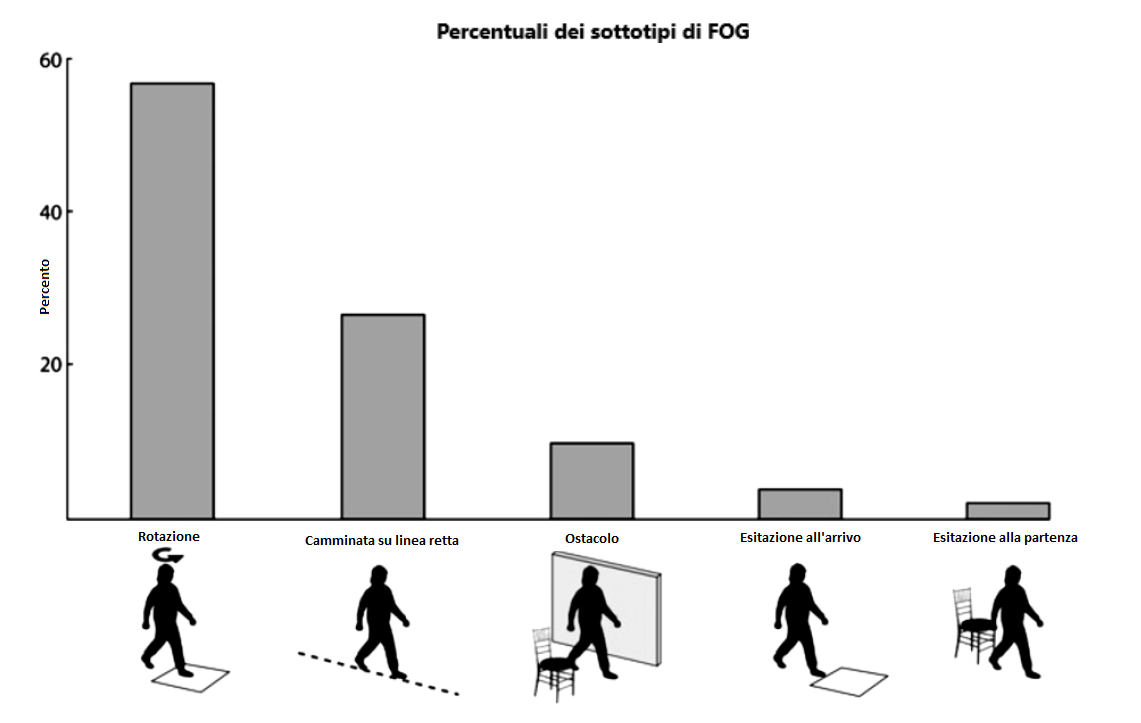
\includegraphics[scale=0.4]{images/Proportion_of_FOG_sub-types.png}
	\caption{Diversi tipi di Freezing esistenti e loro percentuale di incidenza su un certo gruppo di malati di Parkinson. [Fonte: J.M. Shine et al., 2012]}
\end{figure}
Dallo studio di Schaafsma et al.\cite{30} emerge che gli episodi di Freezing possono anche essere suddivisi in ulteriori tre sottotipi andando ad osservare i movimenti delle gambe dei pazienti e applicando la classificazione di Thompson e Marsden (1995):
\begin{enumerate}
	\item FoG associato a passi molto piccoli e strascicati con il minimo movimento in avanti (trascinamento con piccoli passi);
	\item FoG caratterizzato da tremore alle gambe, ma nessun movimento in avanti efficace (tremito da fermo);
	\item FoG caratterizzato da acinesia completa, vale a dire, nessun movimento osservabile delle gambe.
\end{enumerate}
La necessità di dividere il FoG in sottogruppi dipende dal fatto che questi ultimi potrebbero avere origine differente e quindi essere provocati da cause separate.
\subsection{Influenza del FoG nella camminata}
Il Freezing of Gait influenza il pattern del cammino sia all’inizio della deambulazione sia a regime incrementando o diminuendo in modo evidente i valori dei parametri sopra riportati. Ad esempio, nei parkinsoniani che manifestano frequenti fenomeni di Freezing, la variabilità della durata del passo risulta maggiore e la lunghezza del passo minore rispetto alle situazioni in cui il Freezing è assente. Inoltre, la velocità e la lunghezza dei primi tre passi sono significativamente inferiori nei pazienti con malattia di Parkinson e con Freezing rispetto ai soggetti sani. Anche se il Freezing è tipicamente considerato un problema motorio, il fatto che spesso compaia quando il paziente si trova in spazi ristretti, suggerisce che la percezione dello spazio contribuisce in larga misura a scatenare il sintomo\cite{37}.Inoltre, i pazienti con Freezing hanno velocità media del cammino minore rispetto a pazienti sani e subiscono una riduzione ulteriore della velocità nel momento in cui si trovano a dover attraversare una porta o uno spazio stretto. Depressione e ansia possono comportare un carico cronico sulla salute mentale, e la depressione è associata con i cambiamenti di andatura, tra cui una maggiore variabilità passo-a-passo. Il Dual-Tasking, l’ansia e la depressione possono incrementare la variabilità del passo, la di-sincronizzazione di gamba destra e sinistra e l'asimmetria nei pazienti con Parkinson riducendo così la soglia per il FoG. \\
\begin{figure}[]
	\centering
	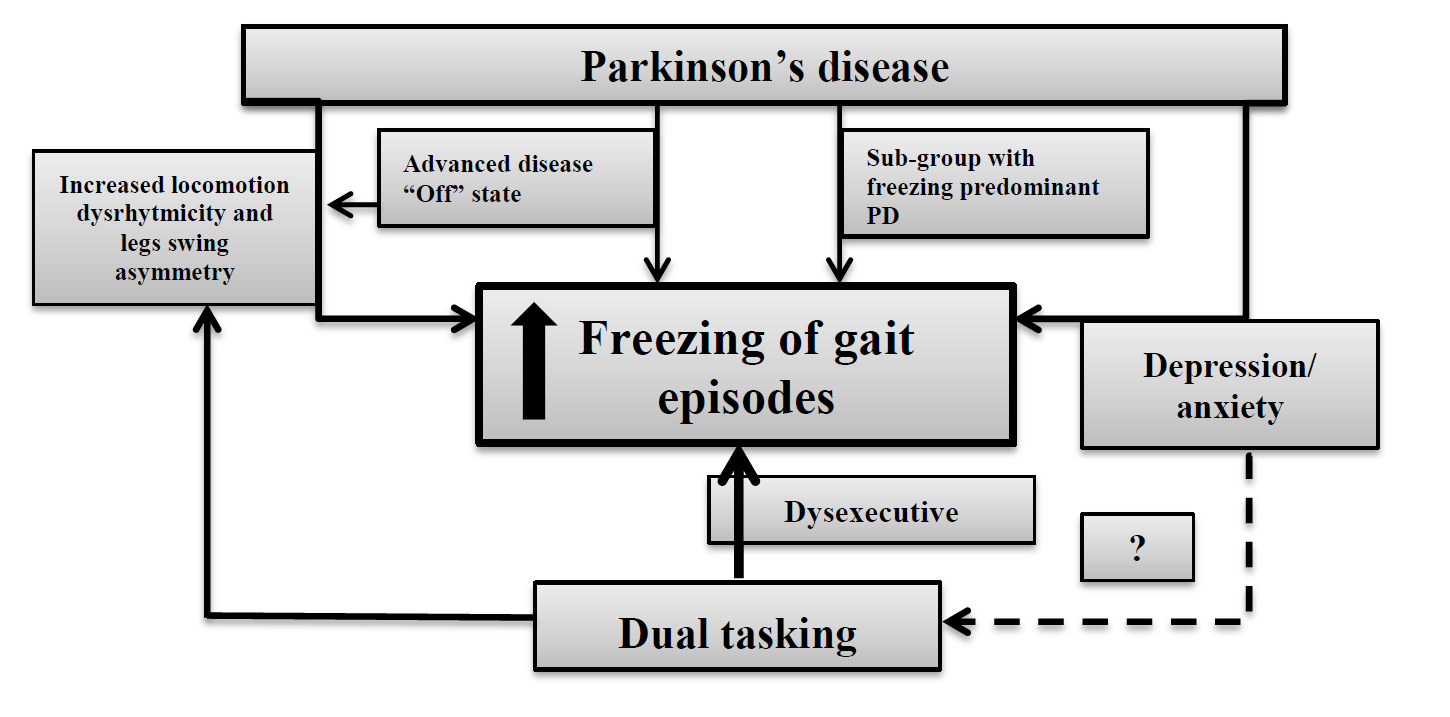
\includegraphics[scale=0.4]{images/Schema_Concettuale_Stress.png}
	\caption{Quadro concettuale relativo al Freezing of Gait (FoG) riguardante aspetti mentali e motori.}
\end{figure}

\section{Machine Learning}
Il Machine Learning si occupa della realizzazione di sistemi che si basano su osservazioni o esempi come dati per la sintesi di nuova conoscenza (classificazioni, generalizzazioni, riformulazioni). Il Machine Learning (ML) o Apprendimento automatico è una disciplina scientifica che progetta e sviluppa algoritmi che consentono agli elaboratori di evolvere il proprio comportamento basandosi su dati empirici. Il principale obiettivo di ricerca in ambito di Machine Learning è “imparare” a riconoscere automaticamente pattern complessi ed effettuare scelte intelligenti basandosi su dati già analizzati. La necessità di ricorrere al ML nasce dal fatto che prevedere a priori l'intero set di possibili comportamenti in base all'input, costruendo per esempio manualmente un set di regole, è troppo complesso da descrivere in un linguaggio di programmazione. Parallelamente, la difficoltà di tale metologia risiede nell'incertezza con cui si individua una corrispondenza tra input e output: essa si basa su un meccanismo parametrico per la generazione dei dati, di cui però non si conoscono a priori valori esatti dei parametri.\\
Caratteristica del ML è l'induzione, ossia l’estrazione di leggi generali a partire da un insieme di dati osservati. Essa si contrappone alla deduzione in cui, a partire da leggi generali, si prevede il valore di un insieme di variabili. L’induzione parte dall’osservazione per misurare un insieme di variabili e per poi effettuare previsioni su ulteriori dati. Questo processo complessivo nel quale, a partire da un insieme di osservazioni, si vuole effettuare previsioni su nuovi dati prende il nome di inferenza.\\
Gli algoritmi di apprendimento automatico sono tradizionalmente divisi in tre principali tipologie:
\begin{itemize}
	\item \textbf{Apprendimento supervisionato}: quando l'utente fornisce esempi (e controesempi) di quello che si deve apprendere. E' il problema più studiato	nel machine learning. Esso si pone l’obiettivo di prevedere, dato un
	elemento di cui si conoscono un insieme di parametri (features), il valore di un diverso parametro di output relativo all’elemento stesso;
	\item \textbf{Apprendimento non supervisionato}: parte da osservazioni non preclassificate;
	\item \textbf{Apprendimento con rinforzo}: tecnica di programmazione che si basa sul 	presupposto che l'algoritmo possa ricevere stimoli dall'esterno a seconda
	delle scelte fatte.
\end{itemize}
Il problema del ML è definito a partire da un universo di elementi: ciascun elemento x è descritto dai valori assunti da un insieme di features considerate come input del problema. Ad ogni x è associato un valore y di output (o target). A partire dalla conoscenza di un insieme T di elementi (denominato training set) in cui ogni elemento è descritto da una coppia ($x_i$ ,$y_i$), con $x_i$ = vettore dei valori delle d features $x_{i1}, x_{i2}, ... , x_{id}$ e $y_i$ = valore di output, si vuole derivare un modello delle relazioni sconosciute tra features e valori di output, che, dato un nuovo elemento x, consenta di predire il corrispondente valore di output y. 
\begin{figure}[]
	\centering
	\includegraphics[scale=0.8]{images/Tipologie_Machine_Learning.png}
	\caption{Schema delle tipologie di Machine Learning}
\end{figure}
Lo scopo dell'apprendimento supervisionato è di costruire un \textbf{modello di predizioni} basato su evidenze in presenza di incertezze. Un algoritmo di apprendimento supervisionato prende un insieme conosciuto di dati di input e di risposte ai dati (output) ed allena un modello al fine di generare predizioni ragionevoli a nuovi dati di input. Esistono due tecniche per questo approccio:
\begin{itemize}
	\item \textbf{Classificazione}: tecnica per predire risposte discrete, classificando i dati di input in categorie;
	\item \textbf{Regression}: tecnica per predirre risposte continue.
\end{itemize}
L'apprendimento non supervisionato, invece, trova pattern nascosti o strutture intrinseche nei dati. Tale tecnica è usata per identificare inferenze da un dataset consistente di dati di input senza classi già definite. Il clustering è l'approccio più diffuso di tale tecnica ed è utilizzato per trovare gruppi nei dati.\\
Con il ML difficilmente c'è una strada diretta dall'inizio alla fine della progettazione, ma si continua ad iterare e provare idee ed approcci differenti. Per questo è importante definire uno schema di lavoro generale ed evidenziare alcuni punti di decisione chiave lungo il percorso:
\begin{enumerate}
	\item Accesso e caricamento dei dati: questi possono essere di tutte le forme e i tipi, incompleti o mescolati;
	\item Pre-processamento dei dati: applicazione di filtri o ri-campionamento;
	\item Derivazione di feature:trovare caratteristiche peculiari a partire dai dati;
	\item Allenamento del modello di ML: può essere un procedimento lungo, poichè dipende da molti parametri;
	\item Integrazione del modello in un sistema di produzione.
\end{enumerate}
\begin{figure}[]
	\centering
	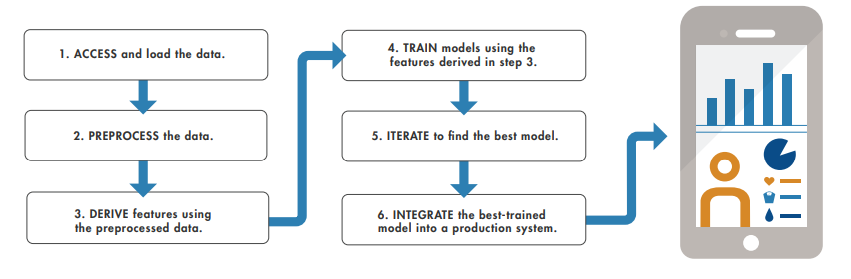
\includegraphics[scale=0.8]{images/Workflow_ML.png}
	\caption{Esempio di Workflow tramite Machine Learning}
\end{figure}
La scelta della modalità supervised o unsupervised si basa sui vantaggi e svantaggi di entrambe: la modalità supervised riesce a predire la giusta classe per le istanze appartenti al test set ma richiede una consistente quantità di istanze annotate e
questo può rappresentare un processo costoso se effettuato manualmente. La modalità unsupervised tipica del clustering, invece, ha il vantaggio di non richiedere un training già annotato (situazione particolarmente frequente quando si
ricorre al ML) ma difficilmente etichetta correttamente il cluster e ottiene una precisione più scarsa rispetto al primo metodo nell'associare le istanze ai cluster corretti. 

\subsection{Cluster Analysis}
Con il termine Cluster Analysis, o analisi dei gruppi, si intendono le procedure che permettono di individuare, all'interno di un insieme di oggetti di qualsiasi natura, alcuni sottinsiemi, \textbf{clusters} appunto, mutuamente esclusivi e tendenzialmente omogenei al loro interno. Le tecniche di Cluster Analysis creano i gruppi in modo tale che ogni osservazione sia molto simile a tutte le altre che appartengono allo stesso gruppo, in funzione di alcuni criteri prestabiliti. Alla fine del procedimento, i cluster finali dovrebbero esibire un'alta omogeneità interna (intra-cluster) ed un'alta eterogeneità esterna (inter-cluster), quindi gli oggetti all'interno dei cluster saranno vicini tra loro, mentre gli oggetti che appartengono a differenti cluster saranno più lontani tra loro.\\
La cluster analysis rientra tra le tecniche di tipo esplorativo e pertanto non è necessaria alcuna assunzione a priori, anche se impone una serie di decisioni durante l'analisi:
\begin{itemize}
	\item Scelta delle variabili;
	\item Criteri di similarità o distanza;
	\item Tecniche di aggregazione;
	\item Numero dei gruppi da ottenere;
	\item Valutazione della qualità della soluzione;
	\item Scelta fra le diverse possibili soluzioni.
\end{itemize}
\begin{figure}[]
	\centering
	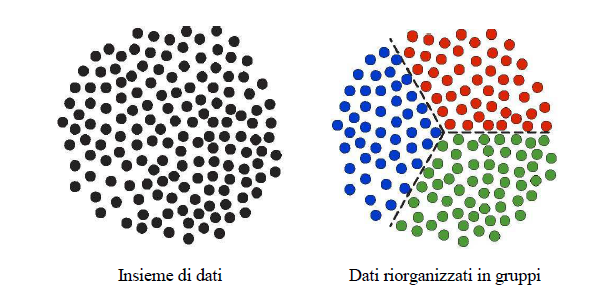
\includegraphics[scale=0.8]{images/Esempio_Cluster.png}
	\caption{Rappresentazione dei dati e dei gruppi ottenuti con la cluster analysis}
\end{figure}
Per classificare e raggruppare gli elementi in gruppi omogenei, è necessario introdurre una nozione di prossimità o similarità. Un indice di prossimità tra due generici elementi $x_i$ e $x_j$ è definito come una funzione dei rispettivi vettori riga nella matrice dei dati: $IP_{ij} = f(x_{i}^{'},x_{j}^{'}) i,j=1,2,..,n$. Due individui sono vicini quando la loro dissimilarità o distanza è piccola o, equivalentemente, quando la loro similarità è grande. Le principali misure di similarità sono illustrate in tabella \ref{TAB:SIMILARITA'}.
\begin{figure}[h!]
	\centering
	%\scriptsize
	\begin{tabular}{ l || c || c || }
		\multicolumn{1}{l||}{Tipo di dato} &  
		\multicolumn{1}{c||}{Misura} &
		\multicolumn{1}{c||}{Formula}\\
		\hline
		\hline
		Binario					&	Coefficiente di Sokal		&	$S_{ij}=(a+d)/(a+b+c+d)$	\\
		Binario					&	Coefficiente di Jaccard		& 	$S_{ij}=a/(a+b+c)$\\
		Categorici non binari	& 	Media delle variabili		&	$S_{ij}=(1/p) \sum_{k=1}^{p} s_{ijk}$\\
		Dati Continui			& 	Distanza Euclidea			&	$d_{ij}=[\sum_{k=1}^{p}(x_{ik}-x_{jk})^2]^{1/2}$\\
		Dati Continui			& 	Distanza City Block			&	$d_{ij}=\sum_{k=1}^{p}|x_{ik}-x_{jk}|$\\
		
	\end{tabular}
	\vspace{0.1cm}
	\caption{Misure di Similarità}
	%\vspace{-0.2cm}
	\label{TAB:SIMILARITA'}
\end{figure}
\\
I principali algoritmi di clustering sono:
\begin{itemize}
	\item \textbf{K-means}: l'obiettivo che l'algoritmo si prepone è di minimizzare la varianza totale intra-cluster. Ogni cluster viene identificato mediante un centroide o punto medio. L'algoritmo segue una procedura iterativa. Inizialmente crea K partizioni e assegna ad ogni partizione i punti d'ingresso o casualmente o usando alcune informazioni euristiche. Quindi calcola il centroide di ogni gruppo. Costruisce quindi una nuova partizione associando ogni punto d'ingresso al cluster il cui centroide è più vicino ad esso. Quindi vengono ricalcolati i centroidi per i nuovi cluster e così via, finché l'algoritmo non converge;
	\item \textbf{K-medoids}: è molto simile al k-means, con la sola condizione che il centroide deve corrispondere ad un elemento;
	\item \textbf{Gerarchico}: produce insiemi nidificati di clusters analizzando la similarità tra coppie di oggetti e raggruppando gli elementi in un albero binario gerarchico. Ne esistono di due tipi: agglomerativo, ossia ogni elemento è un cluster e si uniscono tra di loro fino ad arrivare ad unico cluster, e divisivo, nel quale, all'inizio, ho un unico grande cluster che poi viene diviso;
	\item \textbf{Self-Organizing Map}: sono reti neurali a connessioni laterali dove i neuroni di uscita sono organizzati in griglie di bassa dimensione (2D o 3D). Ogni ingresso è connesso a tutti i neuroni di uscita e ad ogni neurone è associato un vettore dei pesi della stessa dimensione dei vettori d'ingresso. La dimensione del vettore d'ingresso è generalmente molto più alta della dimensione della griglia di uscita;
	\item \textbf{Fuzzy C-means}: molto simile anch'esso al K-means, con la sola condizione che un elemento può appartenere a più di un cluster contemporaneamente;
	\item \textbf{Gaussian Mixture Models}: è un modello probabilistico utilizzato per modellare distribuzioni complesse di dati: l’idea base del modello è quella di suddividere un generico dataset di dati(popolation) in diverse partizioni (subpopolation) e rappresentare queste ultime attraverso una funzione di densità di probabilità. L’obiettivo è quindi rappresentare un segnale complesso attraverso una combinazione lineare di semplici distribuzioni di probabilità (Mixture Model) utilizzando, come si può intuire dal nome stesso del modello, un insieme di gaussiane per la modellazione di distribuzioni complesse di dati.
\end{itemize}
\begin{figure}[]
	\centering
	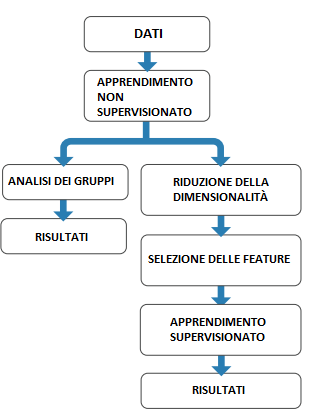
\includegraphics[scale=0.8]{images/Approcci_Clustering.png}
	\caption{Rappresentazione dei possibili approcci usando strategie di clustering}
\end{figure}
\subsection{Classificazione}
I principali approcci di classificazione sono due. In un modello parametrico, il modello stesso è preventivamente caratterizzato da un vettore X di parametri: si suppone quindi che esista una relazione tra features e input e che tale relazione sia rappresentabile all’interno di una famiglia di
relazioni parametriche rispetto a X che costituisce un modello; in altre parole, un'assegnazione di valori al vettore X definisce una specifica relazione della famiglia. Gli elementi nel training set sono utilizzati proprio per derivare tale
assegnazione di valori ai parametri (o una distribuzione di probabilità per tali valori), dopo di che non sono più utilizzati. In un modello non parametrico, invece, il numero di parametri cresce con la dimensione del training set: sostanzialmente, ogni singola previsione, in questo caso, richiede l’utilizzo dell’intero training set. Un esempio di approccio non parametrico sono i classificatori di tipo nearest neighboor, in cui si determina l'elemento $x_i$ del training set più vicino a x e si impone il valore della nuova previsione y associata a x uguale al valore $y_i$ dell’elemento $x_i$.\\
I principali algoritmi di classificazione sono:
\begin{itemize}
	\item \textbf{Decisione Tree}: si tratta di un classificatore con struttura ad albero, in cui ogni nodo può essere o foglia o nodo interno: se foglia, indica il valore della classe assegnata all'istanza; se nodo interno, specifica il test effettuato su un attributo. Per ciascun valore assunto da un attributo in un test, l'algoritmo crea un ramo ed il relativo sottoalbero. Il focus principale dell'algoritmo di crescita del decision tree è come scegliere gli attributi da testare in ciascun nodo interno dell'albero. L'obiettivo è selezionare gli attributi più utili per classificare le istanze di training
	attraverso una strategia top down, che consiste in una ricerca greedy degli
	attributi senza tornare a riconsiderare le precedenti scelte. Il criterio di split (suddivisione) con cui crea un nuovo nodo si basa sul massimo guadagno di informazione (info gain). In pratica sceglie l'attributo che riesce a dividere “meglio” le istanze appartenenti a classi diverse (detto anche criterio di massima riduzione di incertezza). Quando tutti gli elementi in un nodo hanno la medesima classe, l'algoritmo non procede con ulteriore split (criterio di stopping).
	\item \textbf{K-Nearest-Neighbors}: esso memorizza le istanza del training, poi, basandosi su un criterio di vicinanza, mette in relazione l'istanza da classificare con alcune istanze del training set presenti nello spazio delle feature.  In pratica, l'istanza è classificata “a maggioranza” in base alla
	classe più comune tra le k istanze più vicine del training. Tutto il lavoro è fatto dal classificatore in runtime. Data una nuova istanza x da classificare, il classificatore cerca i k esempi del training che sono più “simili” a x e
	guarda le loro etichette. Qualsiasi label ricorra più frequentemente tra le k label più vicine è scelta per assegnare la classe a x.
	\item \textbf{Support Vector Machine}:  l'idea principale di questo classificatore consiste nel rappresentare gli esempi del training come punti nello spazio mappati in modo tale che punti appartenenti a classi differenti siano separati dal più ampio gap possibile. I punti che mappano il test set saranno assegnati ad una categoria o all'altra in base al lato del gap su cui cadono. Più specificatamente, SVM costruisce un iperpiano ed esegue una buona separazione quando l'iperpiano ha la più ampia distanza dai punti di training più vicini di ciascuna classe. Ci sono molti iperpiani che potrebbero classificare il dato. La miglior scelta è quella di selezionare l'iperpiano che rappresenta la più ampia separazione, o margine, tra due classi, ossia l'iperpiano tale che la distanza tra esso e il punto più vicino su ciascun lato sia massima.
\end{itemize}
\subsection{Validazione della Classificazione}
Al fine di valutare la bontà della classificazione effettuata, viene introdotto il concetto di \textbf{Matrice di Confusione}. Essa è una matrice nxn, con n=numero di classi, nella quale vengono messe a confronto le etichette reali con quelle del classificatore proposto. La figura \ref{immagine_matrice_confusione_2classi}  rapprestra la matrice di confusione con 2 classi possibili:
\begin{itemize}
	\item Il \textbf{Veri Positivi} indica quante volte ho classificato giusto l'etichetta che io considero come positiva, ad esempio la classe 1;
	\item Il \textbf{Veri Negativi} indica quante volte ho classificato giusto l'etichetta che io considero come negativa, ad esempio la classe 2;
	\item Il \textbf{Falsi Positivi} indica quante volte ho classificato sbagliato l'etichetta che io considero come positiva, ossia il mio classificatore ha etichettato il mio campione con la classe 1, ma in realtà quella misurazione appartiene alla classe 2;
	\item Il \textbf{Falsi Negativi} indica quante volte ho classificato sbagliato l'etichetta che io considero come negativa, ossia il mio classificatore ha etichettato il mio campione con la classe 2, ma in realtà quella misurazione appartiene alla classe 1;
\end{itemize}
\begin{figure}[h!]
	\centering
	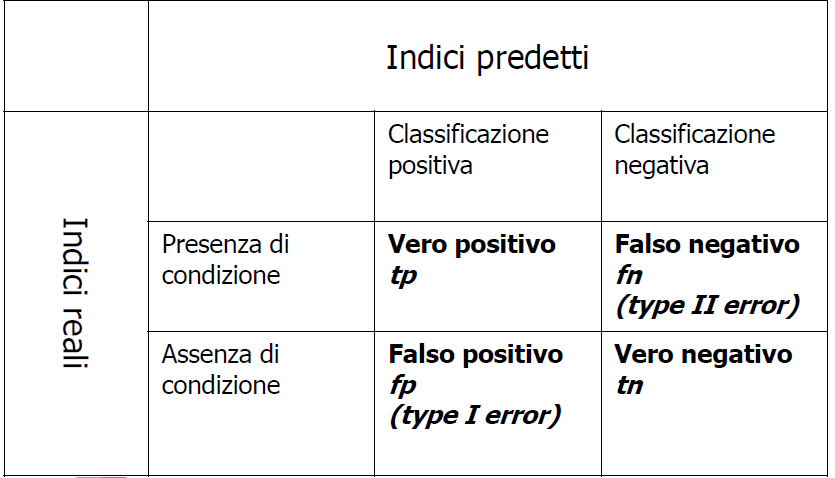
\includegraphics[scale=0.5]{images/matrice_confusione.png}
	\caption{Rappresentazione della matrice di confusione per 2 classi}
	\label{immagine_matrice_confusione_2classi}
\end{figure}
La condizione ideale di classificazione sarebbe quella in cui la matrice di confusione è diagonale, ossia non presento falsi positivi o falsi negativi. Da questa si possono ricavare varie misure, tutte nell'intervallo [0,1]:
\begin{itemize}
	\item \textbf{Accuratezza}: $\dfrac{tp+tn}{tp+tn+fp+fn}$
	\item \textbf{Precisione}: $\dfrac{tp}{tp+fp}$
	\item \textbf{Sensitività}: $\dfrac{tp}{tp+tn}$
	\item \textbf{F1-measue}: $\dfrac{2*precisione*sensitivita' }{sensitivita' + precisione}$
	\item \textbf{Specificità}: $\dfrac{tn}{fp+tn}$
\end{itemize}
Nel caso di più classi, di possono generalizzare le misure di precisione e sensitività associate alle singole classe, mentre il concetto di accuratezza resta sempre lo stesso. La figura \ref{immagine_matrice_confusione_cclassi} rappresenta la generalizzazione delle formula suddette.
\begin{figure}[h!]
	\centering
	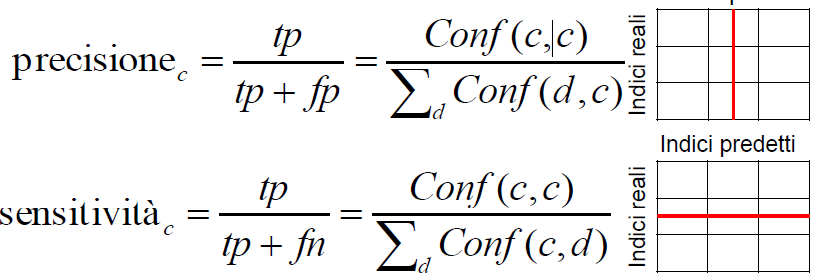
\includegraphics[scale=0.5]{images/matrice_confusione_cclassi.png}
	\caption{Rappresentazione della matrice di confusione per c classi}
	\label{immagine_matrice_confusione_cclassi}
\end{figure}

\section{Riduzione della dimensionalità}
\subsection{Analisi Delle Componenti Principali}
\begin{figure}[]
	\centering
	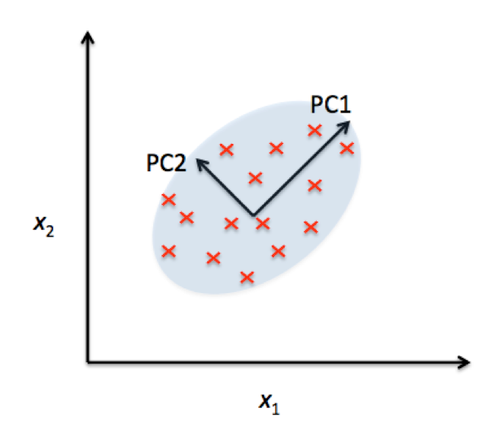
\includegraphics[scale=0.8]{images/pca.png}
	\caption{Rappresentazione del cambio di dimensionalità tramite PCA}
\end{figure}
L'analisi in componenti principali o \textbf{PCA} è una tecnica per la semplificazione dei dati, con lo scopo primario di ridurre un numero più o meno elevato di variabili in alcune caratteristiche latenti. Questo procedimento prende il nome di \textbf{feature reduction}. Ciò avviene tramite una trasformazione lineare delle variabili che proietta quelle originarie in un nuovo sistema cartesiano nel quale la nuova variabile con la maggiore varianza viene proiettata sul primo asse, la seconda variabile per dimensione della varianza sul secondo asse e così via. La riduzione della complessità avviene quindi limitandosi ad analizzare le principali (per varianza) tra le nuove variabili. Diversamente da altre trasformazioni lineari, in questa tecnica sono gli stessi dati che determinano i vettori di trasformazione.\\
Un metodo per calcolare la componente $w_i$ (ossia quella che effettua la trasformazione per la variabile i) utilizza la \textbf{matrice delle covarianze} di x, mentre un altro metodo possibile usa la matrice dei coefficienti di correlazione. Innanzitutto, si devono trovare gli autovalori della matrice di covarianza: Si ottengono così tanti autovalori quante sono le variabili x. L'autovalore con il maggiore valore corrisponde alla dimensione w che ha la maggior varianza: esso sarà dunque la varianza della componente principale numero 1. Per ciascun autovalore viene calcolato il corrispondente autovettore , ossia la matrice dei coefficienti che moltiplicano le vecchie variabili x nella combinazione lineare per l'ottenimento delle nuove variabili w. La matrice degli autovettori degli autovettori viene definita anche matrice di rotazione V e, eseguendo l'operazione $W = V*X $, dove W è il vettore colonna avente come elementi le nuove variabili $w_1,w_2,..$ e X è il vettore colonna avente come elementi le vecchie variabili $x_1,x_2,..$, si possono trovare le coordinate di ciascun punto nel nuovo spazio vettoriale. Alla fine, quindi, si tengono solo le componenti le quali, sommate tra di loro, esprimono una certa varianza (es. 90\% della varianza dei dati), mentre le altre vengono ignorate. In questo modo, partendo da n variabili iniziali, posso arrivare a (n-k) nuove variabili, dove k è il numero di componenti che non mi servono per raggiungere la soglia di varianza prefissata.
\subsection{Analisi dei Discriminanti Lineari}
Mentre la PCA è utile per la rappresentazione dei pattern (es. riconoscimento di immagini), l'analisi dei discriminanti lineari o \textbf{LDA} viene usata per discriminare tali pattern, ossia per trovare delle misure che mi permettano di dividere in più classi i miei dati. Entrambe vengono usate per la riduzione della dimensionalità delle variabili di input).\\
L'obiettivo della LDA è quello di trovare un vettore w, di traformazione, tale per cui classi differenti siano ben separate, mentre la diffusione di ogni classe sia ridotta il più possibile. In pratica, si tratta di trovare una soluzione al cosidetto criterio di Fisher: \begin{equation} J_F = \dfrac{w^TS_Bw}{w^TS_ww}  \end{equation}, nella quale $S_B$ ed $S_W$ sono rispettivamente la matrice di dispersione tra le classi e la matrice di dispersione all'interno della classe. Nel caso di due classi, la $S_B$ si calcola come: \begin{equation} S_B = (m_1 - m_2)(m_1 - m_2)^T \end{equation}, dove $m_1$ rappresenta la media della classe 1 e $m_2$ quella della classe 2. $S_w$, invece, si calcola come \begin{equation}S_W = \sum_{i=1}^{c} \sum_{x \in w_i}^{} (x - m_i)(x-m_i)^T\end{equation} con $m_i$ = media della classe i e c = numero di classi.\\
La soluzione del criterio di Fisher viene chiamata anche \textbf{Problema dell'Autovalore Generalizzato} e viene rappresentata da tale equazione: \begin{equation}S_Bw=\lambda S_ww\end{equation} e, se $S_w$ è invertibile, diventa \begin{equation}S_w^{-1}S_Bw=\lambda w\end{equation}, corrispondente al problema degli autovalori regolari che coinvolge $S_W^{-1}S_B$. Una volta che w viene trovato, le feature cercate vengono calcolate: \begin{equation}y = w^Tx\end{equation} le quali possono essere usate per allenare l'algoritmo di classificazione scelto e procedere alla predizione su nuovi dati.\\
Nel caso si abbiano più di 2 classi, la matrice di dispersione tra le classi, la quali misura la separazione tra le classi, diventa: \begin{equation}S_B=\sum_{i=1}^{c} n_i(m_i-m)(m_i-m)^T\end{equation} con $n_i$ = numero di campioni di training appartenenti alla classe i ed m = media di tutti i campioni di training. Ci saranno quindi C-1 autovettori, ognuno proveniente da una soluzione di (3.5), che potrebbero non essere ortogonali tra loro ma formano uno sottospazio lineare tale per cui il criterio di Fisher è massimizzato. Questi vengono inseriti in una matrice W e si calcolano le feature come in (3.6). 
\begin{figure}[]
	\centering
	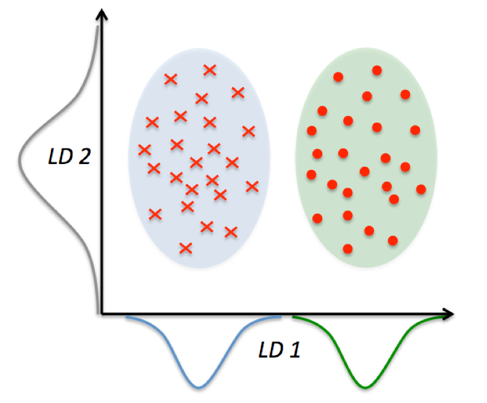
\includegraphics[scale=0.8]{images/lda.png}
	\caption{Rappresentazione del cambio di dimensionalità tramite LDA}
\end{figure}

% !TEX root = ../main.tex
% ---------------------------------------------------------------
% GOALS
% ---------------------------------------------------------------

\chapter{Motivations and Goals}\label{chap4:Goals}

% !TEX root = ../main.tex

% ---------------------------------------------------------------
% Automatic generation of a self-adaptive TLM model
% ---------------------------------------------------------------

\chapter[Apprendimento non supervisionato]{Identificazione dei contesti di preFOG}\label{chap5:Automatic}
Il flusso della tesi viene rappresentato in figura \ref{FlussoTesi}.\\
\begin{figure}[]
	\centering
	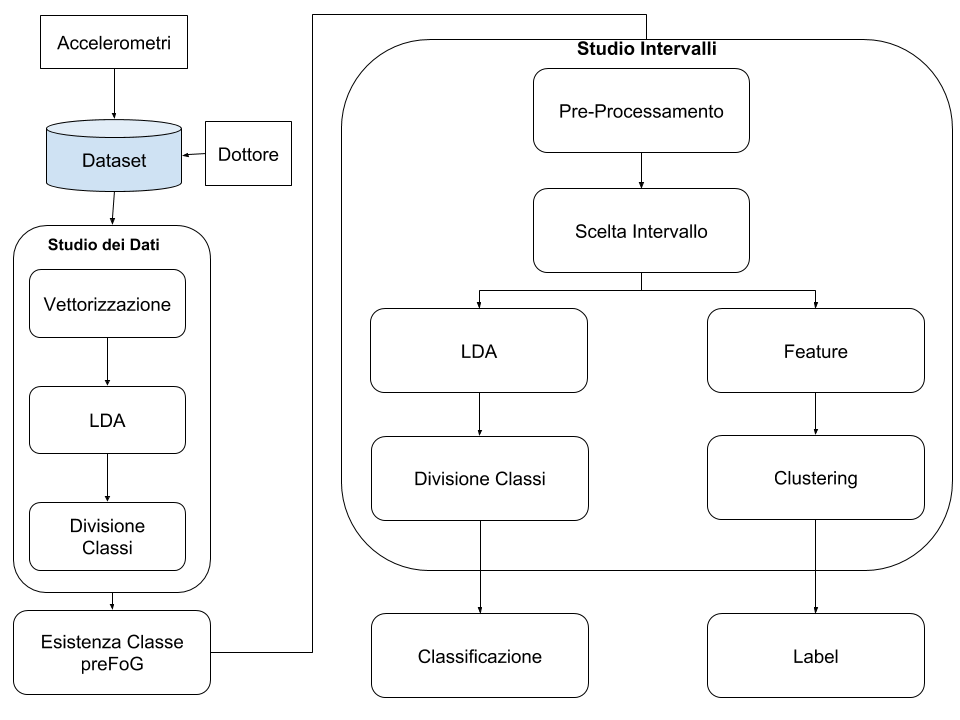
\includegraphics[scale=0.35]{images/FlussoTesi.png}
	\caption{Rappresentazione del flusso della tesi}
	\label{FlussoTesi}
\end{figure}
Lo sviluppo della procedura é stato svolto usando software Matlab.

\section{Studio sull'esistenza della classe preFOG}
Nel lavoro svolto in questa tesi si vogliono usare 3 classi invece delle 2 fornite dal dataset. Il primo passo dunque é quello di dimostrare che effettivamente le 3 classi sono distinte tra loro e che quindi sviluppare un approccio basandosi su tali classi é possibile.\\
Per fare questo, si é usato un approccio di Discriminazione Lineare. Un discriminante é una funzione che prende in ingresso un vettore x e lo assegna ad una tra le K classi fornite. Il metodo di discriminazione che si vuole usare é quello di Fisher, il quale viene spiegato nella sezione \ref{Fisher}.\\
\subsection{Divisione dei dati}
Per ogni paziente, prendiamo in input la matrice di dati grezzi degli accelerometri fornita dal dataset, la quale contiene anche un campo relativo al tempo di ogni campione ed un'etichetta, che mi indica lo stato in cui si trova il mio paziente. Dividiamo i dati degli accelerometri da quelli relativi al tempo ed allo stato e calcoliamo delle feature su tali dati. Queste vengono calcolate vettorizzando finestre di dati grezzi, ossia prendendo tutte le righe e colonne della finestra e disponendole lungo un vettore riga.  Ogni nuova finestra non comincia dalla fine della precedente, ma presenta una certa sovrapposizione. Per tenere traccia dell'etichetta reale a cui ogni finestra temporale appartiene, abbiamo usato il vettore relativo all'etichetta fornita dal dataset e, per ogni finestra temporale, abbiamo tenuto quella che si presenta più volte all'interno di essa. Il codice implementativo di quanto appena descritto é fornito in \ref{vettorizzazione}.
\begin{lstlisting}[style=Matlab-editor,frame=single, caption=Vettorizzazione dei dati degli accelerometri, label=vettorizzazione]
for i=1:size_windows_sample-size_overlap_samples:m - size_windows_sample
B = A(i:i+size_windows_sample-1,:);
% vettorizzo ogni finestra
B=B(:);
F(number_sample,:)=B';


%salvo la classe di ogni finestra
class(number_sample)=mode(FREEZE(i:i+size_windows_sample-1,:));

%go to next sample
number_sample = number_sample + 1;

end
\end{lstlisting}
\subsection{Algoritmo di discriminazione}
Una volta vettorizzato l'intero dataset, si procede ad applicare l'algoritmo di discriminazione, il quale per prima cosa divide le feature appena calcolate tramite le classi di appartenenza. Calcola quindi la media per ogni classe e determina la dimensione di ognuna di esse. A questo punto, ricava la within class covariance e la between class covariance, ossia quanta similarità esiste tra gli elementi della stessa classe e quanta dissimilarità è presente tra classi differenti. Una volta trovate tali misure, prende gli autovalori ed autovettori della soluzione del problema dell'autovalore generalizzato e tiene solo quelli più rappresentativi, che nel caso dell'approccio di Fisher sono pari al numero di classi presenti meno 1. Questi autovalori vengono poi moltiplicati per le feature calcolate precedentemente per ottenere una riduzione della dimensionalità' ed avere 2 feature rappresentative. Il codice della discriminazione viene fornito in \ref{code_LDA}.
\begin{lstlisting}[style=Matlab-editor,frame=single, caption=LDA, label=code_LDA]
A=F';

%quindi ho A 1152x1449 double
%1152 finestre
%ogni finestra ha 1449 features
[d,N] = size(A);

K =  max(class); % numero classi in gioco;

% 1. Divido le feature tramite le classi Ck
for k = 1:K
a = find (class == k);
Ck{k} = A(:, a);
end

% 2. Calcolo la media per ogni classe per ogni finestra
for k = 1:K
mk{k} = mean(Ck{k},2);
end
% 3. Determino la grandezza di ogni classe
for k = 1:K
[d, Nk(k)] = size(Ck{k});
end
% 4. determino le within class covariance
for k = 1:K
S{k} = 0;
for i = 1:Nk(k)
S{k} = S{k} + (Ck{k}(:,i)-mk{k})*(Ck{k}(:,i)-mk{k})';
end
S{k} = S{k}./Nk(k);
end
Swx = 0;
for k = 1:K
Swx = Swx + S{k};
end

% 5. determino la between class covariance
% 5.1 determino la media totale
m = mean(A,2);
Sbx = 0;
for k=1:K
Sbx = Sbx + Nk(k)*((mk{k} - m)*(mk{k} - m)');
end
Sbx = Sbx/K;

MA = inv(Swx)*Sbx;

% eigenvalues/eigenvectors
[V,D] = eig(MA);

% 5: transform matrix
if (k > 1)
W = V(:,1:K-1);
end
if (k == 1)
W = V(:,1:1);
end

% 6: transformation
Y = W'*A;
\end{lstlisting}


\section{Approccio non supervisionato ed intervalli}
In letteratura, la finestra temporale su cui vengono calcolate le feature é stata presa molte volte a priori, basandosi su delle ipotesi. Non é mai stato presentato uno studio su quale possa essere il miglior intervallo di divisione dei dati per calcolare le feature. Quello che ci prefissiamo in questa sezione é dunque testare diverse combinazioni di durata delle finestre con sovrapposizione al fine di trovare quella che meglio divide i nostri dati. Allo stesso tempo, usando tale studio,usiamo di algoritmi di clustering al fine di cercare di sostituire il dottore nella fase di etichettatura dei dati.  L'approccio che è stato preso in considerazione è basato sul calcolo di feature (o proprietà) derivanti dalla matematica statistica. Il flusso di tale approccio è:
\begin{enumerate}
	\item Pre-processamento dei dati degli accelerometri, al fine di eliminare il rumore presente ed identificare eventuali punti di outline, ossia campioni che non presentano affinità col resto dei dati poiché dovuti a movimenti non consoni;
	\item Finestramento dei dati in base ad intervalli variabili al fine di calcolare le feature, dove ogni intervallo presenta una certa sovrapposizione con l'intervallo precedente;
	\item Calcolo effettivo delle feature statistiche;
	\item Applicazione degli algoritmi di clustering;
	\item Calcolo di metriche che indicano quanto bene gli algoritmi di clustering hanno diviso i dati in relazione alle label fornite dal dataset.
\end{enumerate}
\begin{figure}[h!]
	\centering
	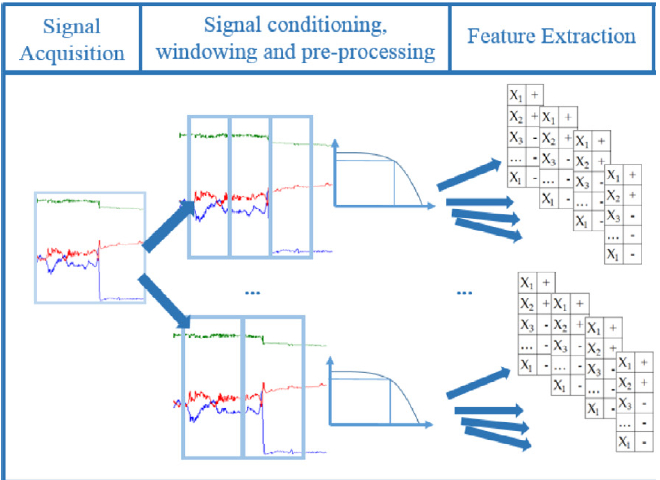
\includegraphics[scale=0.6]{images/flusso_feature.png}
	\caption{Schema generale di calcolo delle feature statistiche}
	\label{Flusso Feature}
\end{figure}
\subsection{Pre-processamento dei dati}
Gli accelerometri sono dispositivi che misurano le vibrazioni o l'accelerazione del movimento di una struttura. La forza generata dalle vibrazioni o una variazione del movimento (accelerazione) fa in modo che la massa "comprima" il materiale piezoelettrico, che genera una carica elettrica proporzionale alla forza esercitata su di esso. Dato che la carica è proporzionale alla forza e che la massa è una costante, la carica è proporzionale anche all'accelerazione. Come tutti i dispositivi che misurano delle grandezze presentano dell'incertezza strumentale che può portare ad avere rumore, ossia un segnale non desiderato, di origine naturale o artificiale, che si sovrappone all'informazione degli accelerometri stessi. Questo rumore porta ad avere dei punti definiti outlier, ossia campioni che non presentano affinità col resto dei dati poiché dovuti a movimenti non consoni.\\
Al fine di non alterare in modo negativo il calcolo delle nostre feature, si rende necessario rimuoverli dal nostro dataset. Per identificarli, è stato implementato un filtro passa-alto che elimina tutte le frequenze inferiori a 0.5Hz, le quali non appartengono al normale movimento umano ma indicano appunto la presenza di rumore, come evidenziato in \cite{21}.
\subsection{Definizione degli intervalli}
Una volta filtrati i dati, il passo successivo dell'algoritmo consiste nel dividerli in intervalli temporali, al fine di poter computare le caratteristiche degli stessi. Un intervallo contiene un determinato movimento, che però verrebbe "interrotto" con la fine della finestra stessa e quindi potrei perdere informazioni su tale movimento. Per evitare il più possibile tale perdita, viene usato un approccio che sfrutta le sovrapposizioni tra intervalli, per cui ogni nuova finestra non inizia subito dopo la fine della precedente, ma all'interno di essa. La durata degli intervalli che sono stati presi in considerazione sono:
\begin{itemize}
	\item  Da 1 secondi a 5 secondi per la finestra temporale, con un incremento di 0.5 secondi;
	\item Da 0.5 a 4.5 secondi per l'intervallo di overlap, con un incremento sempre di 0.5 secondi.
\end{itemize}
La condizione fondamentale per usare le sovrapposizioni è che l'intervallo delle stesse non sia mai maggiore della durata delle finestre temporali, per cui è stata posta la condizione che la finestra temporale sia sempre almeno 0.5 secondi più lunga dell'intervallo di sovrapposizione. Per capire da dove parte la nuova finestra, quindi, prendiamo la posizione a cui siamo arrivati e togliamo la durata della sovrapposizione. L'implementazione viene fornita in \ref{intervals}.
\begin{lstlisting}[style=Matlab-editor,frame=single, caption=Definizione degli intervalli, label=intervals]  % Start your code-block
...
for k = 5:5:45

Y = k/10;

for i = (Y+0.5):0.5:5
%dimensione della finestra in secondi
size_windows_sec = i;
%dimensione della finestra in campioni
size_windows_sample = Fs * i;

%dimensione dell'overlap in secondi
size_overlap_sec = Y;
%dimensione dell'overlap in campioni
size_overlap_samples = Fs * Y;

number_sample = 1;

%for each sample window, compute the features
for i=1:size_windows_sample-size_overlap_samples:m - size_windows_sample
B = A(i:i+size_windows_sample-1,:);
...
\end{lstlisting}
\subsection{Calcolo delle Feature}
 Per ogni possibile combinazione di finestra temporale e sovrapposizione, a questo punto vengono calcolate le feature per ogni intervallo. Le feature prese in considerazione nel nostro studio sono descritte in tabella \ref{TAB:Feature}.
\begin{table}[h!]
	\begin{tabular}{ |p{0.05\textwidth} | p{0.25\textwidth} | p{0.6\textwidth} | }
		\multicolumn{1}{|p{0.05\textwidth} |}{\textbf{N}} &  
		\multicolumn{1}{p{0.25\textwidth} |}{\textbf{Feature}} &
		\multicolumn{1}{p{0.6\textwidth} |}{\textbf{Descrizione}}\\
		\hline
		\hline
		1 & Minimo & Valore minimo del segnale\\
		2 & Massimo & Valore massimo del segnale \\
		3 & Mediana & Valore mediano del segnale \\
		4 & Media & Valore medio del segnale \\
		5 & Media Armonica & Media armonica del segnale \\
		6 & Errore Quadratico Medio & Valore Quadratico medio del segnale \\
		7 & Media Geometrica & Media geometrica del segnale \\
		8 & Varianza & Radice della deviazione standard \\
		9 & Deviazione Standard & Deviazione media del segnale rispetto alla media \\
		10 & Curtosi & Allontanamento dalla normalità distributiva del segnale \\
		11 & Simmetria & Grado di asimmetria della distribuzione del segnale \\
		12 & Moda & Il numero che appare più volte nel segnale \\
		13 & Media Tagliata & Media tagliatadel segnale nella finestra \\
		14 & Entropia & Misura della di distruzione delle componenti in frequenza \\
		15 & Range & Differenza tra il valore minimo e massimo del segnale \\
		16 & Magnitudine & Somma della norma euclidea di tre assi normalizzato sulla lunghezza del segnale \\
		17 & Area Magnitudine & Accelerazione della magnitudine di tre assi normalizzato sulla lunghezza del segnale \\
		18 & Autovalori delle direzioni dominanti & Autovalori della matrice di covarianza di tre assi \\
		19 & Accelerazione media dell'energia & Valore medio dell'energia sui 3 assi \\
	\end{tabular}
\caption{Descrizione delle Feature Statistiche}
\label{TAB:Feature}
\end{table}\\
Nel dataset, ogni campione è etichettato. Poiché le nostre feature sono composte da molti campioni messi assieme, si rende necessario trovare un metodo per unire, sbagliando il meno possibile, tutte le etichette della finestra che prendiamo in considerazione. Per fare ciò, si è deciso di utilizzare la funzione di moda, ossia il numero che si ripete più spesso all'interno dell'intervallo considerato. L'etichetta risultante viene inserita nella tabella e verrà utilizzata come criterio di confronto, al fine di valutare le prestazioni degli algoritmi di clustering. L'implementazione del codice è fornito in \ref{extract_feature}
\begin{lstlisting}[style=Matlab-editor,frame=single, caption=Calcolo delle Feature, label=extract_feature]  % Start your code-block
...
%time sample
F(number_sample, 1) = TIME(i,:);
%min --> minimum value for each accelerometer
F(number_sample, 2:10) = min(B);
%max --> maximum value for each accelerometer
F(number_sample, 11:19) = max(B);
%median --> median signal value
F(number_sample, 20:28) = median(B);
%mean --> average value
F(number_sample, 29:37) = mean(B);
%ArmMean --> harmonic average of the signal
F(number_sample, 38:46) = harmmean(B);
%root mean square --> quadratic mean value of the signal
F(number_sample, 47:55) = rms(B);
%variance --> square of the standard deviation
F(number_sample, 56:64) = var(B);
%standard deviation --> mean deviation of the signal compared to the
%average
F(number_sample, 65:73) = std(B);
%kurtosis --> degree of peakedness of the sensor signal distribution
%(allontanamento dalla normalita distributiva)
F(number_sample, 74:82) = kurtosis(B);
%skewdness --> degree of asymmetry of the sensor signal distribution
F(number_sample, 83:91) = skewness(B);
%mode --> number that appears most often in the signal
F(number_sample, 92:100) = mode(B);
%trim mean --> trimmed mean of the signal in the window
F(number_sample, 101:109) = trimmean(B,10);
%range --> difference between the largest and the smallest values of
%the signal
F(number_sample, 110:118) = range(B);
%signal magnitude vector --> sum of the euclidean norm over the three
%axis over the entire window normalized by the windows lenght
F(number_sample, 119) = svmn(B(:,1:3), length(B));
F(number_sample, 120) = svmn(B(:,4:6), length(B));
F(number_sample, 121) = svmn(B(:,7:9), length(B));
%normalized signal magnitude area --> acceleration magnitude summed
%over three axes normalized by the windows length
F(number_sample, 122) = sman(B(:,1:3), length(B));
F(number_sample, 123) = sman(B(:,4:6), length(B));
F(number_sample, 124) = sman(B(:,7:9), length(B));
%eigenvalues of dominant directions --> eigenvalues of the
%covariance matrix of the acceleration data along x, y and z axis
F(number_sample,125) = eigs(cov(B(:,1:3)),1);
F(number_sample,126) = eigs(cov(B(:,4:6)),1);
F(number_sample,127) = eigs(cov(B(:,7:9)),1);
%averaged acceleration energy --> mean value of the energy over
%three acceleration axes
F(number_sample,128) = energyn(B(:,1:3),length(B));
F(number_sample,129) = energyn(B(:,4:6),length(B));
F(number_sample,130) = energyn(B(:,7:9),length(B));
%is freezing?
F(number_sample,131) = mode(FREEZE(i:i+size_windows_sample-1,:));

%go to next sample
number_sample = number_sample + 1;
...
\end{lstlisting}
\subsection{Clustering}
Una volta finestrato il segnale, si procede con l'applicazione degli algoritmi di clustering. Quelli che sono stati presi in considerazione nella nostra analisi sono: K-means, Fuzzy C-Means e Neural Network. Il K-means viene testato in 4 varianti diverse, in base alle seguenti metriche di distanza: cityblock, correlation, cosine, euclidean.\\
Ogni algoritmo di clustering viene applicato in tutte le possibili combinazioni di intervalli ed ognuno di essi restituisce un vettore di numeri, che corrispondono alle etichette che assegnano ad ogni vettore di feature. Questi vengono salvati e verranno poi utilizzati per calcolare le prestazioni degli algoritmi stessi in confronto alla classificazione originale del dottore. L'implementazione del codice è fornita in \ref{clustering}
\begin{lstlisting}[style=Matlab-editor,frame=single, caption=Uso degli algoritmi di clustering, label=clustering]  % Start your code-block
...
            %% k-means %%%

% choose of parameter
means1 = 'sqeuclidean';
means2 = 'correlation';
means3 = 'cityblock';
means4 = 'cosine';
for q=1:4
if q == 1
dist_k = means1;
end
if q == 2
dist_k = means2;
end
if q == 3
dist_k = means3;
end
if q == 4
dist_k = means4;
end
options_km = statset('UseParallel', false);
maxiter = 100000;
% cluster
kidx = kmeans(bonds, numClust, 'distance', dist_k, 'options', options_km, 'MaxIter', maxiter);

P = array2table([A(:,n) kidx]);
writetable(P, [datadir 'versus_kmeans_' dist_k '_' fileruns(r).name] );
display([datadir 'versus_kmeans_' dist_k '_' fileruns(r).name]);
end

%%% neural networks - Self organizing Maps %%%

% Create a Self-Organizing Map
dimension1 = 3;
dimension2 = 1;
net = selforgmap([dimension1 dimension2]);

% Train the network
net.trainParam.showWindow = 0;
[net,tr] = train(net,bonds');

% Test the network
nidx = net(bonds');
nidx = vec2ind(nidx)';

P = array2table([A(:,n) nidx]);
writetable(P, [datadir 'versus_net_' fileruns(r).name] );
display([datadir 'versus_net_' fileruns(r).name]);


%     %%% FUZZY C-MEANS %%%
options(1) = 2;
options(2) = 10000;
options(3) = 1e-5;
options(4) = 0;
% Hide iteration information by passing appropriate options to FCM
[centres,U] = fcm(bonds,numClust,options);
[~, fidx] = max(U);
fidx = fidx';


P = array2table([A(:,n) fidx]);
writetable(P, [datadir 'versus_cmeans_' fileruns(r).name] );
display([datadir 'versus_cmeans_' fileruns(r).name]);
...
\end{lstlisting}
\subsection{Calcolo delle prestazioni}
Ogni algoritmo di clustering, per tutte le combinazioni di finestra ed overlap, fornisce un vettore di etichette. Questo rappresenta la divisione in cluster effettuata dall'algoritmo, i quali andranno confrontati con le etichette reali del dataset. Per fare questo, procediamo al calcolo di metriche quali, in ordine, accuratezza, precisione, sensitività e F1-measure. Per quanto riguarda la precisione, la sensitività e l'F1-measure, esse sarebbero relative ad ogni classe, ma poiché ci interessa indovinare la maggior parte delle volte tutte e 3 le classi, quelle che saranno riportate sono la media dei valori per ogni classe. Il codice implementativo é fornito in \ref{rate}

\begin{lstlisting}[style=Matlab-editor,frame=single, caption=Calcolo delle prestazioni, label=rate]  % Start your code-block
...
% Matrice di confusione
[C,order] = confusionmat(D(:,2),D(:,1));
accuracy = c_accuracy(C);
precision = c_precision(C);
recall = c_recall(C);
F1measure = c_F1measure(precision,recall);

B = [accuracy precision recall F1measure];
E = [E B];

end
Q = [Q ; [e E]];
e = [e [0 0 0 0]];
...
\end{lstlisting}
Viene creata dunque una tabella che riassume, per ogni possibile intervallo, le prestazioni dell'algoritmo, come si vede in \ref{ratecluster1}, \ref{ratecluster2}, \ref{ratecluster3}.
\begin{table}[htp]
	\centering
	\caption{Esempio di tabelle delle prestazioni del clustering}
	\label{ratecluster1}
	\resizebox{\textwidth}{!}{%
	\begin{tabular}{|l|l|l|l|l|l|l|l|l|l|l|l|l|}
		\hline
		& \multicolumn{4}{c|}{Secondi: 1} & \multicolumn{4}{c|}{Secondi: 1.5} & \multicolumn{4}{c|}{Secondi: 2} \\ \hline
		Ov 0.5 & 0,7 & 0,6 & 0,3 & 0,4 & 0,8 & 0,3 & 0,3 & 0,3 & 0,91 & 0,5 & 0,5 & 0,5 \\ \hline
		Ov 1 & 0 & 0 & 0 & 0 & 0,7 & 0,3 & 0,3 & 0,3 & 0,8 & 0,6 & 0,5 & 0,55 \\ \hline
		Ov 1.5 & 0 & 0 & 0 & 0 & 0 & 0 & 0 & 0 & 0,91 & 0,72 & 0,6 & 0,6 \\ \hline
	\end{tabular}%
}
\end{table}
\begin{table}[htp]
	\centering
	\caption{Esempio di tabelle delle prestazioni del clustering}
	\label{ratecluster2}
	\resizebox{\textwidth}{!}{%
	\begin{tabular}{|l|l|l|l|l|l|l|l|l|l|l|l|l|}
		\hline
		& \multicolumn{4}{c|}{Secondi: 2.5} & \multicolumn{4}{c|}{Secondi: 3} & \multicolumn{4}{c|}{Secondi: 3.5} \\ \hline
		Ov 0.5 & 0,7 & 0,3 & 0,3 & 0,3 & 0,4 & 0,1 & 0,2 & 0,17 & 0,46 & 0,32 & 0,4 & 0,35 \\ \hline
		Ov 1 & 0,05 & 0,3 & 0,2 & 0,3 & 0,46 & 0,3 & 0,4 & 0,38 & 0,46 & 0,32 & 0,4 & 0,35 \\ \hline
		Ov 1.5 & 0,75 & 0,2 & 0,2 & 0,2 & 0,8 & 0,3 & 0,3 & 0,3 & 0,46 & 0,32 & 0,4 & 0,35 \\ \hline
		Ov 2 & 0,8 & 0,3 & 0,3 & 0,3 & 0,6 & 0,3 & 0,1 & 0,21 & 0,46 & 0,32 & 0,4 & 0,35 \\ \hline
		Ov2.5 & 0 & 0 & 0 & 0 & 0,81 & 0,26 & 0,24 & 0,25 & 0,7 & 0,3 & 0,2 & 0,26 \\ \hline
		Ov 3 & 0 & 0 & 0 & 0 & 0 & 0 & 0 & 0 & 0,6 & 0,3 & 0,31 & 0,31 \\ \hline
	\end{tabular}%
}
\end{table}
\begin{table}[htp]
	\centering
	\caption{Esempio di tabelle delle prestazioni del clustering}
	\label{ratecluster3}
	\resizebox{\textwidth}{!}{%
	\begin{tabular}{|l|l|l|l|l|l|l|l|l|l|l|l|l|}
		\hline
		& \multicolumn{4}{c|}{Secondi: 4} & \multicolumn{4}{c|}{Secondi: 4.5} & \multicolumn{4}{c|}{Secondi: 5} \\ \hline
		Ov 0.5 & 0,8 & 0,36 & 0,35 & 0,35 & 0,81 & 0,32 & 0,34 & 0,33 & 0,75 & 0,24 & 0,26 & 0,25 \\ \hline
		Ov 1 & 0,76 & 0,21 & 0,28 & 0,26 & 0,79 & 0,32 & 0,34 & 0,31 & 0,79 & 0,3 & 0,3 & 0,3 \\ \hline
		Ov 1.5 & 0,46 & 0,36 & 0,33 & 0,35 & 0,8 & 0,36 & 0,35 & 0,35 & 0,59 & 0,24 & 0,33 & 0,29 \\ \hline
		Ov 2 & 0,41 & 0,33 & 0,44 & 0,39 & 0,76 & 0,21 & 0,28 & 0,26 & 0,26 & 0,79 & 0,32 & 0,34 \\ \hline
		Ov2.5 & 0,59 & 0,24 & 0,33 & 0,29 & 0,46 & 0,36 & 0,33 & 0,35 & 0,35 & 0,8 & 0,36 & 0,35 \\ \hline
		Ov 3 & 0,44 & 0,11 & 0,12 & 0,11 & 0,41 & 0,33 & 0,44 & 0,39 & 0,8 & 0,36 & 0,35 & 0,35 \\ \hline
		Ov 3.5 & 0,78 & 0,23 & 0,33 & 0,28 & 0,75 & 0,24 & 0,26 & 0,25 & 0,76 & 0,21 & 0,28 & 0,26 \\ \hline
		Ov 4 & 0 & 0 & 0 & 0 & 0,79 & 0,3 & 0,3 & 0,3 & 0,75 & 0,24 & 0,26 & 0,25 \\ \hline
		Ov 4.5 & 0 & 0 & 0 & 0 & 0 & 0 & 0 & 0 & 0,79 & 0,3 & 0,3 & 0,3 \\ \hline
	\end{tabular}%
	}
\end{table}


\section{Classificazione del preFOG}
Nella sezione precedente, è stato decritto uno studio degli intervalli temporali che ci ha portati a decidere quale sia la migliore scelta di durata sia per la finestra che per la sovrapposizione al fine di dividere al meglio i dati a nostra disposizione. Dalla figura \ref{LDAALL2.png}, si nota come le classi FoG e NoFoG sono a volte confuse tra di loro, mentre il preFOG è più o meno diviso dalle altre due classi. Ma quest'ultima classe è proprio quella che stiamo studiando ed è quella che ci porterebbe a prevenire le occorrenze di FoG, in quanto, identificandola, avrei il tempo di dare lo stimolo prima dell'avvenuta del FoG, mentre se cerco di identificare solo i Freezing darei lo stimolo uditorio in ritardo in ogni caso. Questo ci porta a provare un primo approccio di classificazione a 2 classi, dove raggruppiamo assieme i dati di FoG e noFoG e teniamo separate le occorrenze di preFOG. L'algoritmo  di classificazione scelto è il K-nearest Neighbours (KNN), spiegato nel capitolo \ref{chap3:background}. Usiamo sempre l'intervallo che è stato dimostrato nella sezione precedente essere quello più affidabile. L'algoritmo verrà testato in due modi:
\begin{itemize}
	\item alleniamo il knn su un paziente singolo, effettuiamo una cross-validation sul classificatore e lo testiamo su dei nuovi dati, ossia che non sono stati inclusi nella  cross-validation;
	\item alleniamo il knn sui dati di tutti i pazienti contemporaneamente ed effettuiamo una cross-validation.
\end{itemize}
La cross-validation è una tecnica statistica utilizzabile in presenza di una buona numerosità del campione osservato o training set. In particolare la k-fold cross-validation consiste nella suddivisione del dataset totale in k parti di uguale numerosità (si chiama anche k-fold validation) e, ad ogni passo, la k-esima parte del dataset viene ad essere il validation dataset, mentre la restante parte costituisce il training dataset. In altre parole, si suddivide il campione osservato in gruppi di egual numerosità, si esclude iterativamente un gruppo alla volta e lo si cerca di predire con i gruppi non esclusi.\\

% !TEX root = ../main.tex

% ---------------------------------------------------------------
% Software Implamentation of metodology
% ---------------------------------------------------------------
\chapter[Risultati]{Risultati Sperimentali}\label{chap6:result}
In questo capitolo, verranno descritti i risultati ottenuti nell'identificazione di contesti di FoG e 

\section{Dataset}
L'approccio che andiamo a proporre è stato testato sul dataset DAPHNET\footnote{www.wearable.ethz.ch/resources/Dataset}, il quale contiene dati collezionati da 10 pazienti parkinsoniani, dei quali 8 presentano contesti di FoG, mentre 2 di loro non ne presentano. I dati sono stati registrati usando 3 accelerometri 3D attaccati alla caviglia, al ginocchio e nella zona lombare del paziente, usando una frequenza di campionamento di 64 Hz.\\
I soggetti hanno completato sessioni da 20-30 minuti ciascuno, consistenti di 3 fasi di camminata:
\begin{enumerate}
	\item Camminata avanti ed indietro lungo una linea retta, con delle rotazioni di 180 gradi;
	\item Camminata casuale con una serie di fermate volontarie e rotazioni di 360 gradi;
	\item Camminata che simula attività di vita quotidiana, tra le quali entrare in stanze ed uscirne, camminare nella cucina, prendersi un bicchiere d'acqua e tornare al punto di partenza.
\end{enumerate}
Le prestazioni motorie variano molto tra i pazienti. Mentre alcuni soggetti hanno mantenuto una camminata regolare durante gli episodi di non FoG, altri hanno camminato molto lentamente ed in modo instabile. L'intero dataset contiene in totale 237 episodi di FoG; la durata di ognuno di essi è tra i 0.5s ed i 40.5s. Il 50\% degli episodi di FoG è durato meno di 5.4s ed il 93.2\% è più corto di 20s. Gli episodi di FoG sono stati identificati da fisioterapisti usando registrazioni video sincronizzate. L'inizio di un episodio di FoG è stato definito come il punto dove la sequenza normale di camminata è stata interrotta, mentre la fine del FoG è stata definita come il momento in cui tale sequenza riprende.

\section{Studio sull'esistenza della classe preFOG}
\subsection{Risultati}
Una volta calcolate le feature discriminanti, per visualizzare se effettivamente esiste una distinzione tra le classi, tracciamo un grafico con queste due grandezze in cui ogni punto viene colorato in base alla reale classe di appartenenza.\\
Le figure \ref{LDAS01} e \ref{LDAS02} fanno notare immediatamente come le feature utilizzate riescono a discriminare abbastanza tra le 3 classi, anche se c'è ancora una certa sovrapposizione tra i dati di classi diverse, almeno usando i dati di un solo paziente.\\
Ogni soggetto, però, ha dei pattern di camminata diversi, quindi posso avere dati molto differenti tra un paziente ed un altro. Abbiamo quindi verificato anche se, utilizzando i dati di tutti i pazienti, la discriminazione lineare riesce ancora a distinguere tra le varie classi.\\
La figura \ref{LDAALL} mostra che, usando i dati di tutti i pazienti assieme, una certa divisione rimane, anche se è molto meno netta rispetto a quella del singolo paziente. Questo comunque ci permette di dire che anche tra pazienti differenti, quindi con pattern di cammino diversi, i dati che sono di preFOG sono abbastanza divisi da quelli di noFoG o FoG, quindi un approccio concentrato su questa nuova classe sembra sensato.

\begin{figure}[]
	\centering
	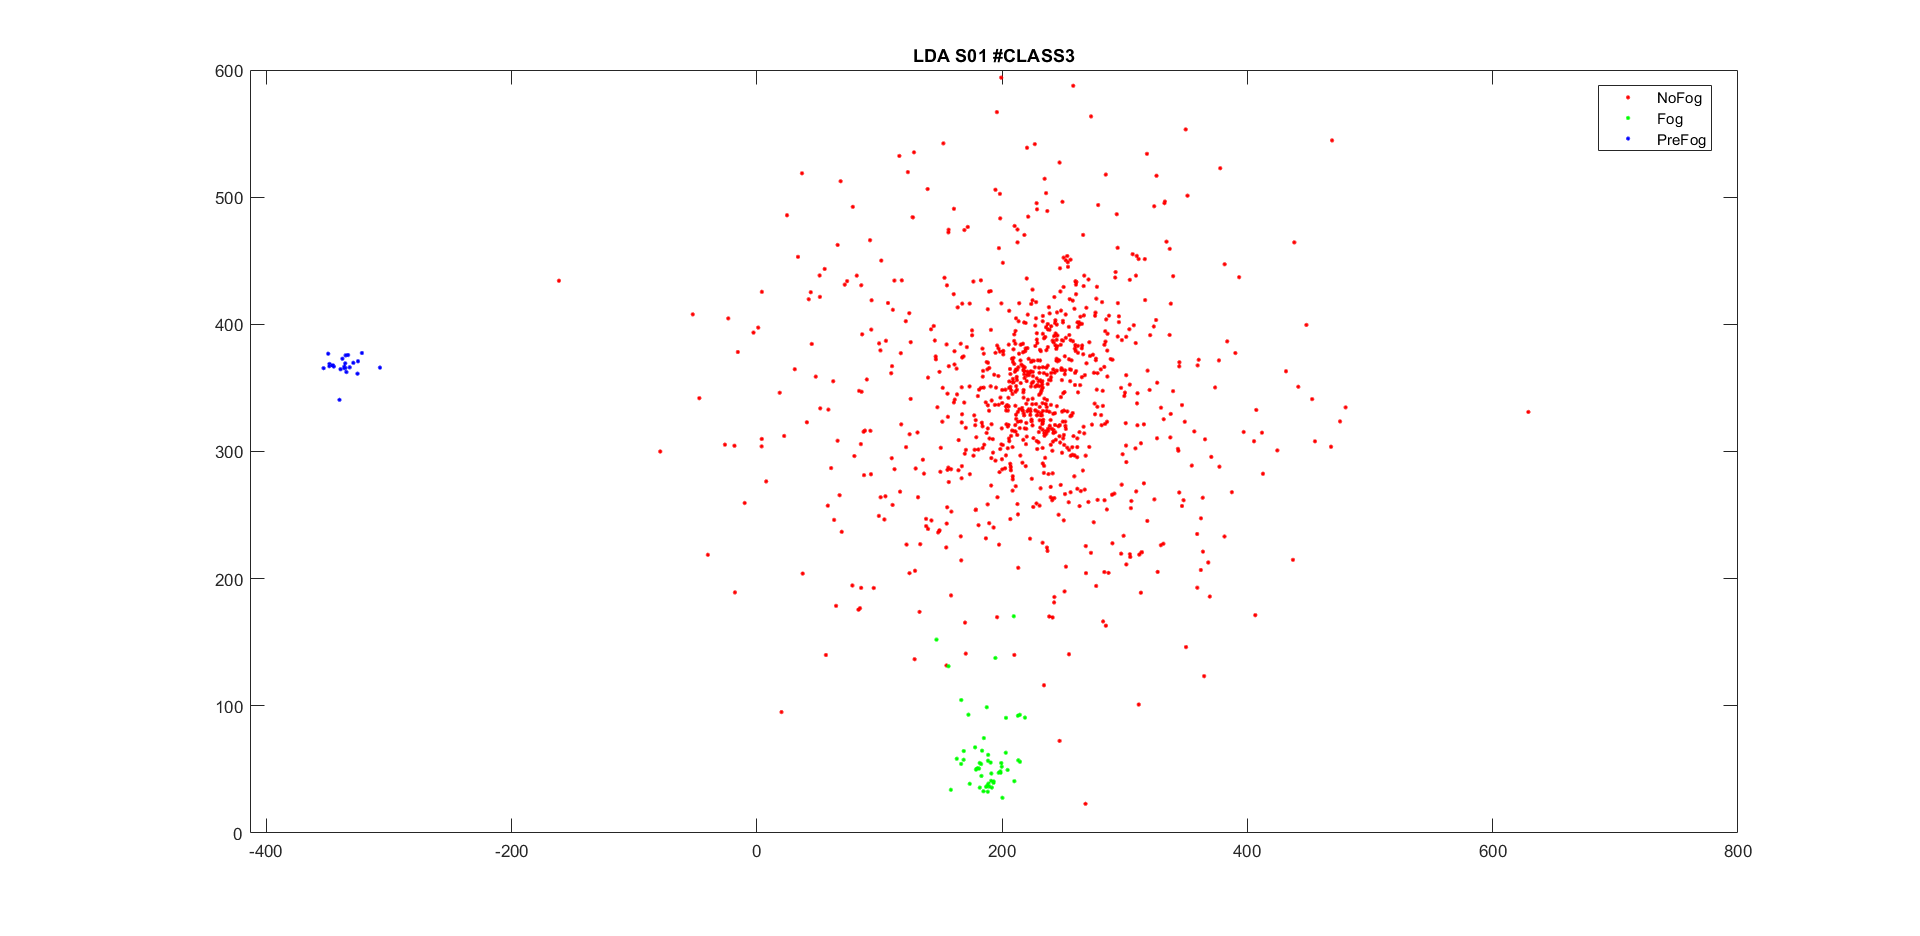
\includegraphics[scale=0.25]{images/LDAS01.png}
	\caption{Grafico delle 3 classi in base alla discriminazione dell'approccio di Fisher per il paziente 1}
	\label{LDAS01}
\end{figure}
\begin{figure}[]
	\centering
	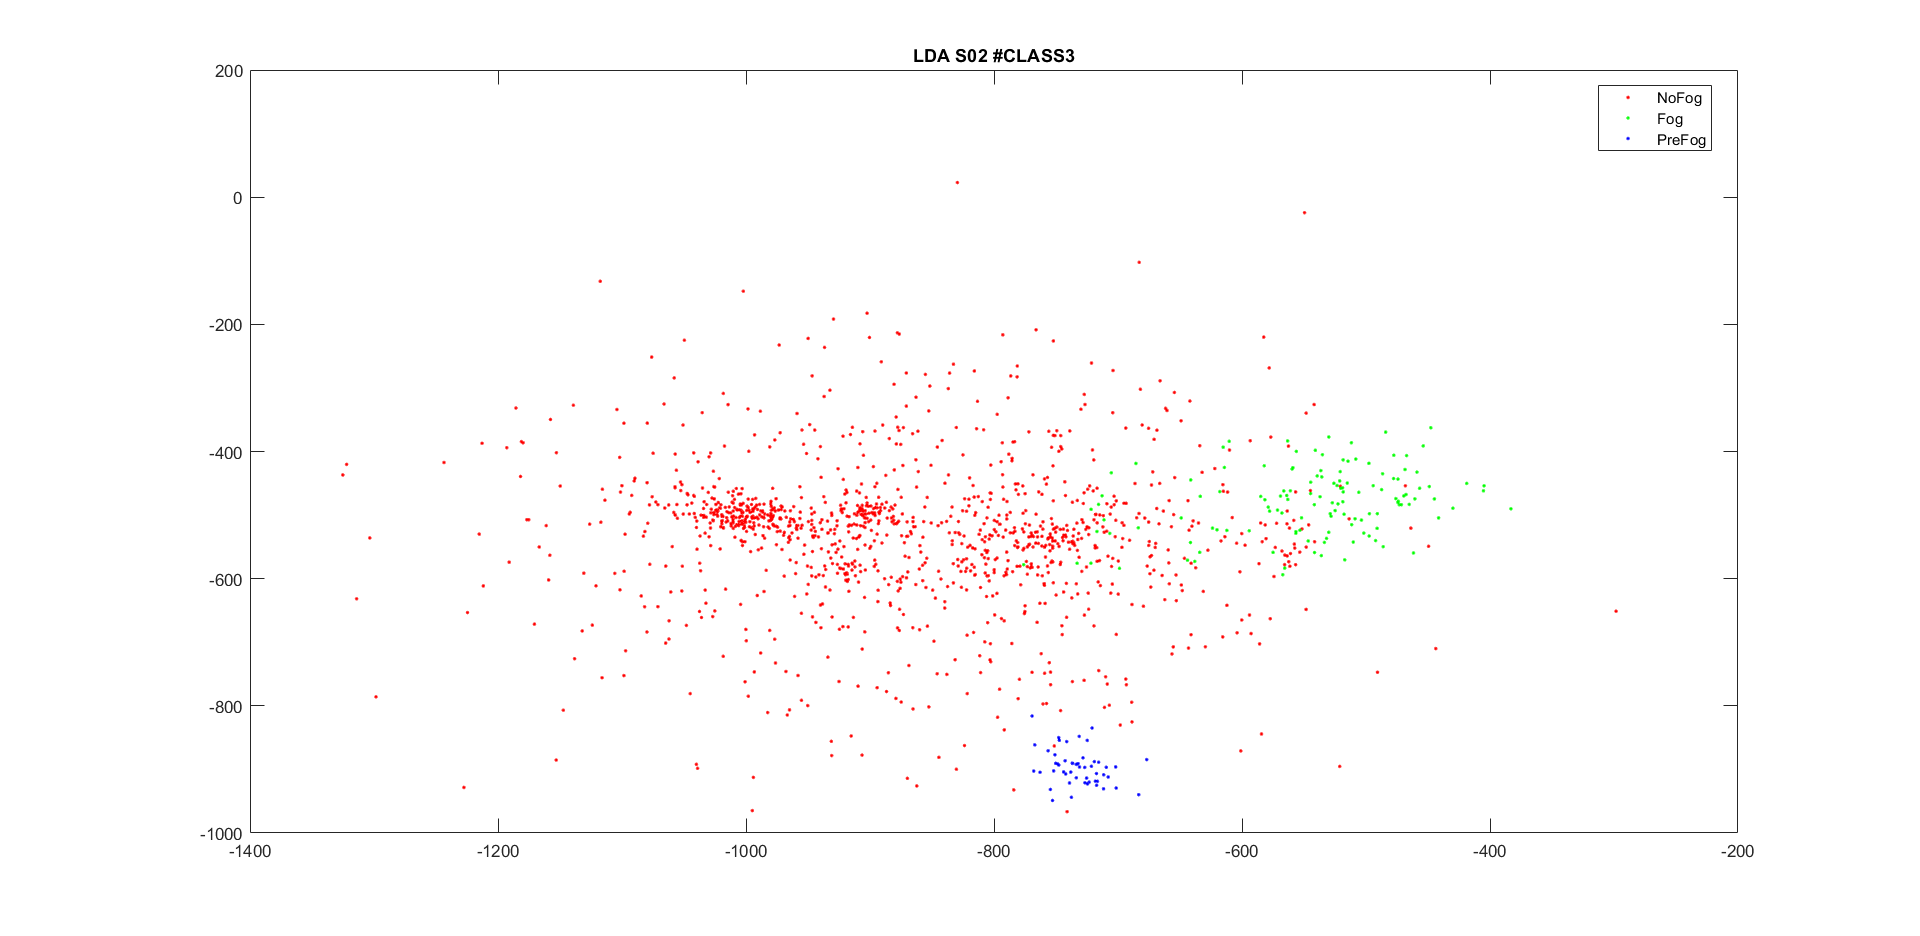
\includegraphics[scale=0.25]{images/LDAS02.png}
	\caption{Grafico delle 3 classi in base alla discriminazione dell'approccio di Fisher per il paziente 2}
	\label{LDAS02}
\end{figure}
\begin{figure}[]
	\centering
	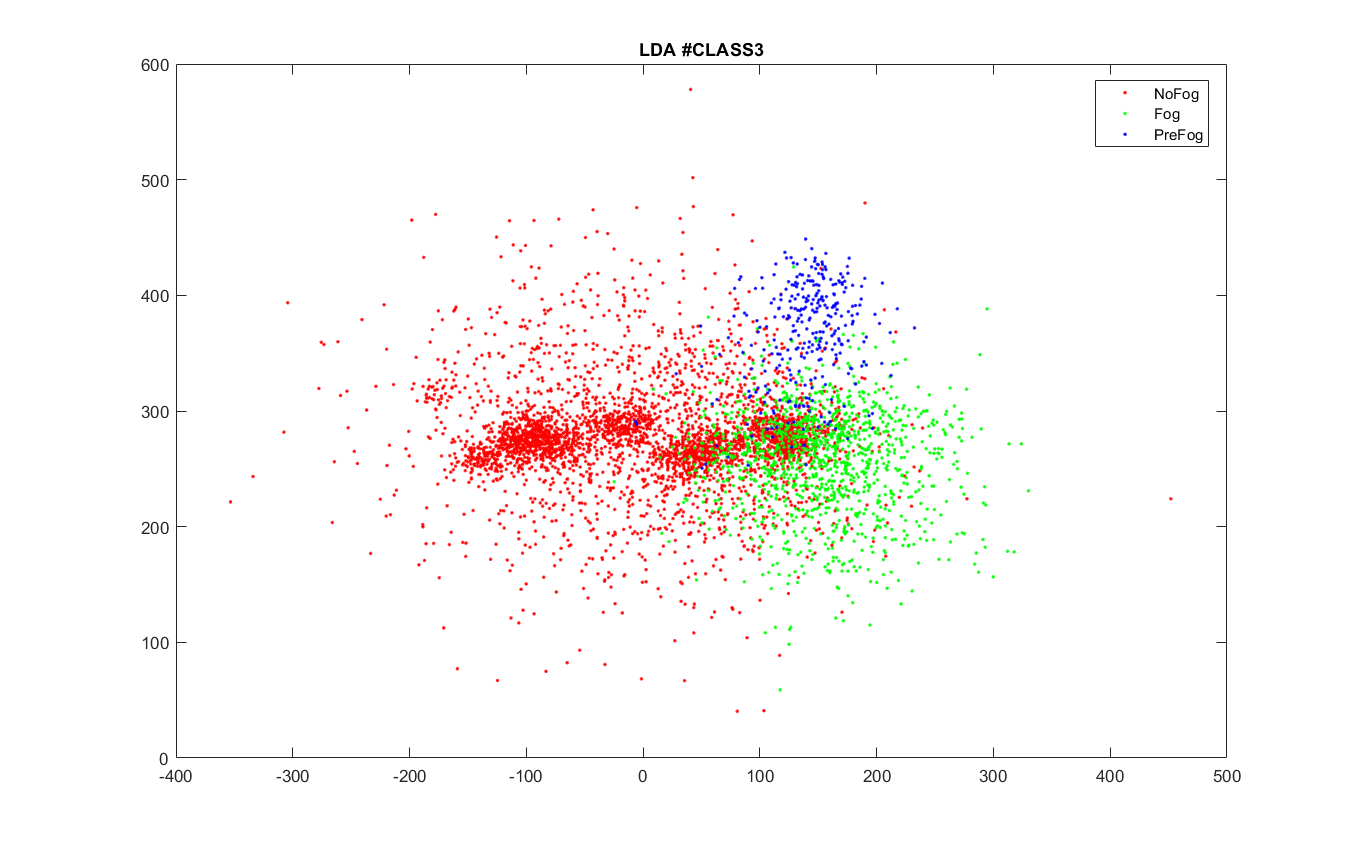
\includegraphics[scale=0.3]{images/LDAALL.png}
	\caption{Grafico delle 3 classi in base alla discriminazione dell'approccio di Fisher presi tutti i pazienti}
	\label{LDAALL}
\end{figure}

\subsection{Risultati Clustering}
Dopo che sono state generate tutte le tabelle, per tutti i pazienti, in cui vengono espressi i valori di accuratezza, precisione, sensitività e F1-measure, siamo interessati all'intervallo migliore, ossia quello che ci fornisce i valori maggiori delle metriche suddette. Per fare questo, analizziamo ogni tabella e, per ogni algoritmo, salviamo l'intervallo ed i valori che presentano le metriche migliori, come nel caso delle tabelle \ref{ratecmeans}, \ref{ratekmeans}, \ref{rateneuralnetwork}. La metrica riportata per il k means é la square euclidean, in quanto é quella che ci ha portato ad i risultati migliori. \\
Ogni tabella descrive:
\begin{itemize}
	\item l'algoritmo di clustering che é stato utilizzato;
	\item il paziente del test;
	\item i valori delle metriche migliori trovate;
	\item la combinazione overlap-secondi in cui risultano tali metriche.
\end{itemize}

% Please add the following required packages to your document preamble:
% \usepackage{graphicx}
\begin{table}[]
	\centering
	\caption{Rate Pazienti per l'algoritmo di clustering C-means}
	\label{ratecmeans}
	\resizebox{\textwidth}{!}{%
		\begin{tabular}{|l|l|l|l|l|l|l|}
			\hline
			\textbf{}         & \multicolumn{6}{c|}{\textbf{CMEANS}}                                                                              \\ \hline
			\textbf{Paziente} & \textbf{Accuratezza} & \textbf{Precisione} & \textbf{Recall} & \textbf{F1} & \textbf{Overlap} & \textbf{Finestra} \\ \hline
			\textbf{S01}      & 0,92                 & 0,31                & 0,33            & 0,32        & 1                & 2                 \\ \hline
			\textbf{S02}      & 0,44                 & 0,46                & 0,63            & 0,53        & 1                & 2                 \\ \hline
			\textbf{S03}      & 0,7                  & 0,51                & 0,57            & 0,54        & 1                & 2                 \\ \hline
			\textbf{S04}      & 0,7                  & 0,33                & 0               & 0           & 0,5                & 1               \\ \hline
			\textbf{S05}      & 0,53                 & 0,49                & 0,46            & 0,47        & 1                & 1,5               \\ \hline
			\textbf{S06}      & 0,57                 & 0,36                & 0,32            & 0,34        & 1                & 1,5               \\ \hline
			\textbf{S07}      & 0,48                 & 0,37                & 0,43            & 0,4         & 1                & 1,5               \\ \hline
			\textbf{S08}      & 0,41                 & 0,39                & 0,43            & 0,41        & 1,5              & 2                 \\ \hline
			\textbf{S09}      & 0,59                 & 0,35                & 0,37            & 0,36        & 1                & 1,5               \\ \hline
			\textbf{S10}      & 0,73                 & 0,33                & 0               & 0           & 0,5                & 1               \\ \hline
		\end{tabular}%
	}
\end{table}

% Please add the following required packages to your document preamble:
% \usepackage{graphicx}
\begin{table}[]
	\centering
	\caption{Rate Pazienti per l'algoritmo di clustering K-means}
	\label{ratekmeans}
	\resizebox{\textwidth}{!}{%
		\begin{tabular}{|l|l|l|l|l|l|l|}
			\hline
			\textbf{Tutti}    & \multicolumn{6}{c|}{\textbf{KMEANS}}                                                                              \\ \hline
			\textbf{Paziente} & \textbf{Accuratezza} & \textbf{Precisione} & \textbf{Recall} & \textbf{F1} & \textbf{Overlap} & \textbf{Finestra} \\ \hline
			\textbf{S01}      & 0,92                 & 0,72                & 0,34            & 0,46        & 1,5              & 2                 \\ \hline
			\textbf{S02}      & 0,82                 & 0,61                & 0,34            & 0,44        & 1                & 2                 \\ \hline
			\textbf{S03}      & 0,75                 & 0,78                & 0,54            & 0,64        & 1,5              & 2                 \\ \hline
			\textbf{S04}      & 1                    & 0,33                & 0               & 0           & 0,5                & 1               \\ \hline
			\textbf{S05}      & 0,67                 & 0,56                & 0,33            & 0,42        & 1                & 2                 \\ \hline
			\textbf{S06}      & 0,91                 & 0,3                 & 0,33            & 0,32        & 1                & 1,5               \\ \hline
			\textbf{S07}      & 0,92                 & 0,31                & 0,33            & 0,32        & 1                & 2                 \\ \hline
			\textbf{S08}      & 0,7                  & 0,57                & 0,34            & 0,42        & 1                & 1,5               \\ \hline
			\textbf{S09}      & 0,81                 & 0,6                 & 0,34            & 0,43        & 1                & 2                 \\ \hline
			\textbf{S10}      & 1                    & 0,33                & 0               & 0           & 0,5                & 1,5               \\ \hline
		\end{tabular}%
	}
\end{table}

% Please add the following required packages to your document preamble:
% \usepackage{graphicx}
\begin{table}[]
	\centering
	\caption{Rate Pazienti per l'algoritmo di clustering Self-Organizing Map}
	\label{rateneuralnetwork}
	\resizebox{\textwidth}{!}{%
		\begin{tabular}{|l|l|l|l|l|l|l|}
			\hline
			\textbf{Tutti}    & \multicolumn{6}{c|}{\textbf{NEURAL NETWORK}}                                                                      \\ \hline
			\textbf{Paziente} & \textbf{Accuratezza} & \textbf{Precisione} & \textbf{Recall} & \textbf{F1} & \textbf{Overlap} & \textbf{Finestra} \\ \hline
			\textbf{S01}      & 0,92                 & 0,31                & 0,33            & 0,32        & 1                & 1,5               \\ \hline
			\textbf{S02}      & 0,81                 & 0,44                & 0,34            & 0,38        & 1                & 1,5               \\ \hline
			\textbf{S03}      & 0,75                 & 0,78                & 0,54            & 0,63        & 1                & 2                 \\ \hline
			\textbf{S04}      & 0,64                 & 0,33                & 0               & 0           & 0,5                & 1                 \\ \hline
			\textbf{S05}      & 0,58                 & 0,42                & 0,46            & 0,44        & 1                & 2                 \\ \hline
			\textbf{S06}      & 0,57                 & 0,32                & 0,31            & 0,31        & 1                & 1,5               \\ \hline
			\textbf{S07}      & 0,63                 & 0,3                 & 0,26            & 0,28        & 1                & 2                 \\ \hline
			\textbf{S08}      & 0,56                 & 0,69                & 0,38            & 0,49        & 1,5              & 2                 \\ \hline
			\textbf{S09}      & 0,57                 & 0,37                & 0,41            & 0,39        & 1                & 2                 \\ \hline
			\textbf{S10}      & 1                    & 0,33                & 0               & 0           & 0,5                & 1               \\ \hline
		\end{tabular}%
	}
\end{table}
\subsection{LDA con intervallo migliore}
In \ref{LDAS01} e \ref{LDAS02} si era notato come esiste una certa distinzione tra le classi, ma restava una sovrapposizione tra alcuni dati di esse, il che ci porta a studiare quale sia il miglior intervallo di divisione dei dati. Analogamente al procedimento per la fase di clustering, iteriamo l'algoritmo di LDA cambiando la durata della finestra temporale e la sovrapposizione tra di essi. Gli intervalli possibili, come nel caso del clustering, vanno da 1 a 5 secondi per la finestra, da 0.5 a 4.5 secondi per la sovrapposizione.\\
Dopo aver provato tutte le possibili combinazioni, risulta anche in questo caso che scegliendo 2 secondi di finestra ed 1 secondo di overlap si ottiene una divisione molto più netta per il singolo paziente, come si può vedere in \ref{LDAS01_best.png} e \ref{LDAS02_best.png}.\\
Anche usando i dati di tutti i pazienti si può notare, in figura \ref{LDAALL2.png}, che c'è un miglioramento nella divisione dei dati, soprattutto considerando il preFOG, usando un intervallo di 2 secondi per la finestra ed 1 secondo per l'overlap.
\begin{figure}[]
	\centering
	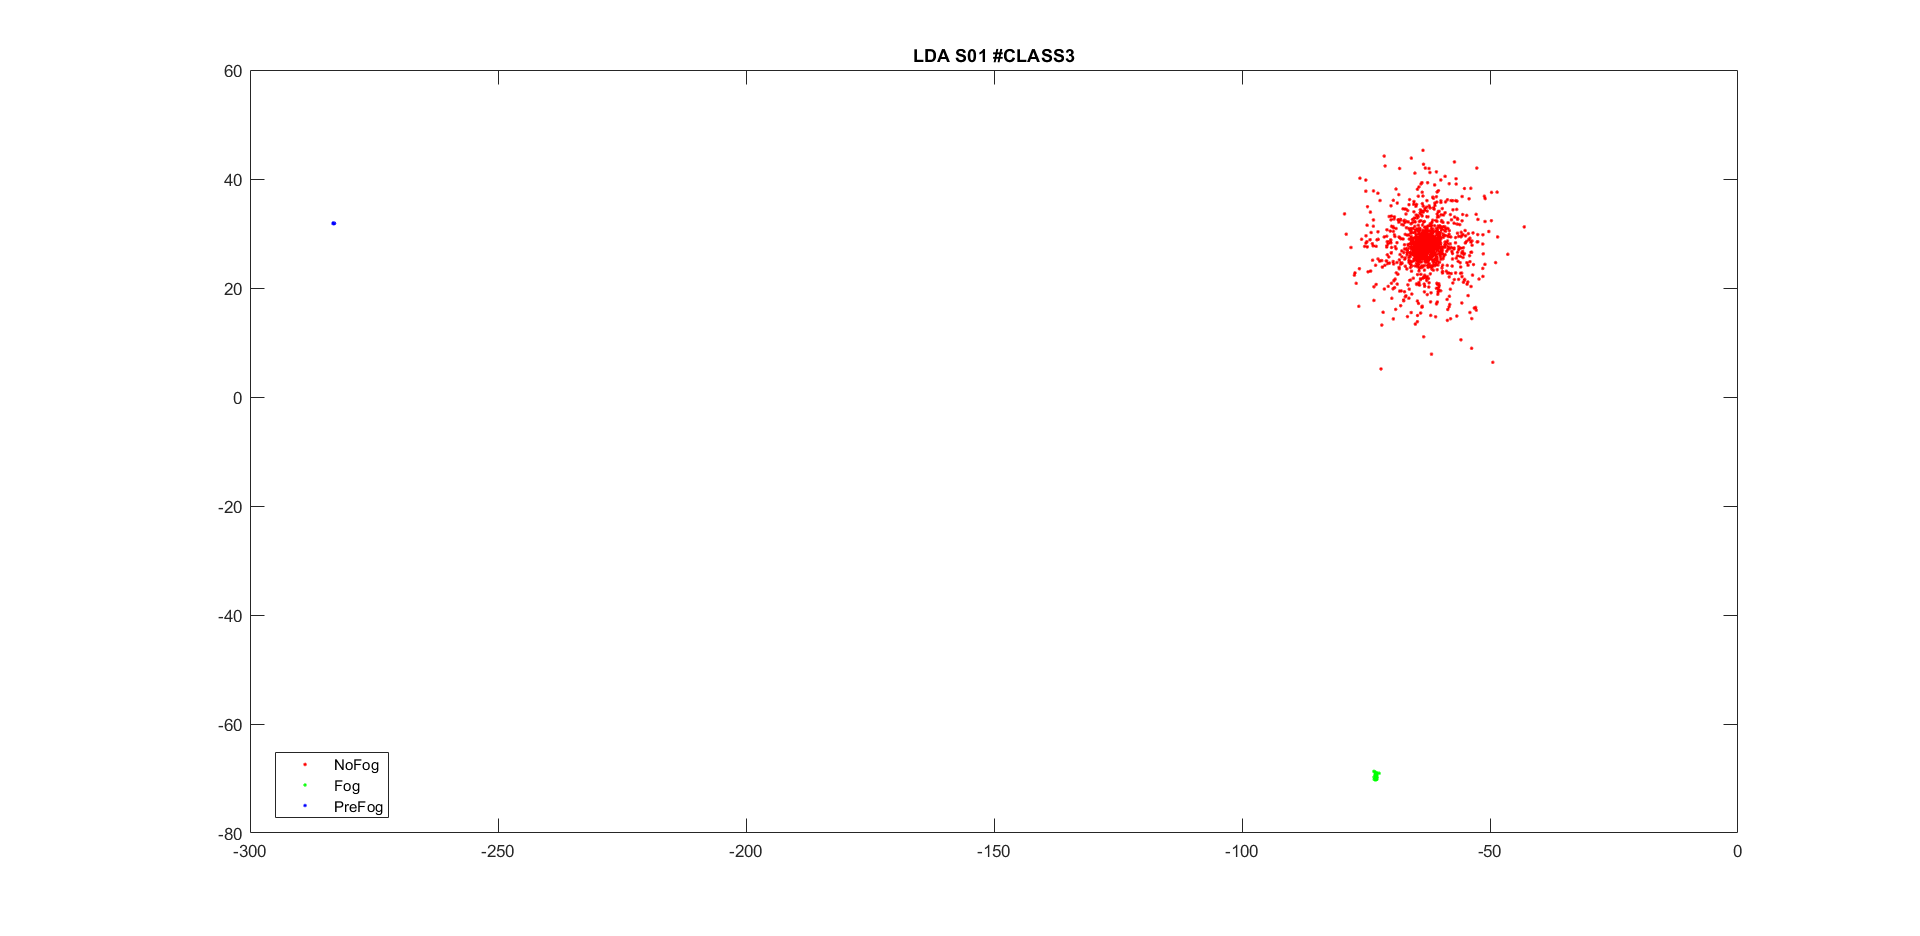
\includegraphics[scale=0.25]{images/LDAS01_best.png}
	\caption{Grafico delle 3 classi in base alla discriminazione dell'approccio di Fisher per il paziente 1 con 2 secondi di finestra ed 1 secondo di overlap}
	\label{LDAS01_best.png}
\end{figure}
\begin{figure}[]
	\centering
	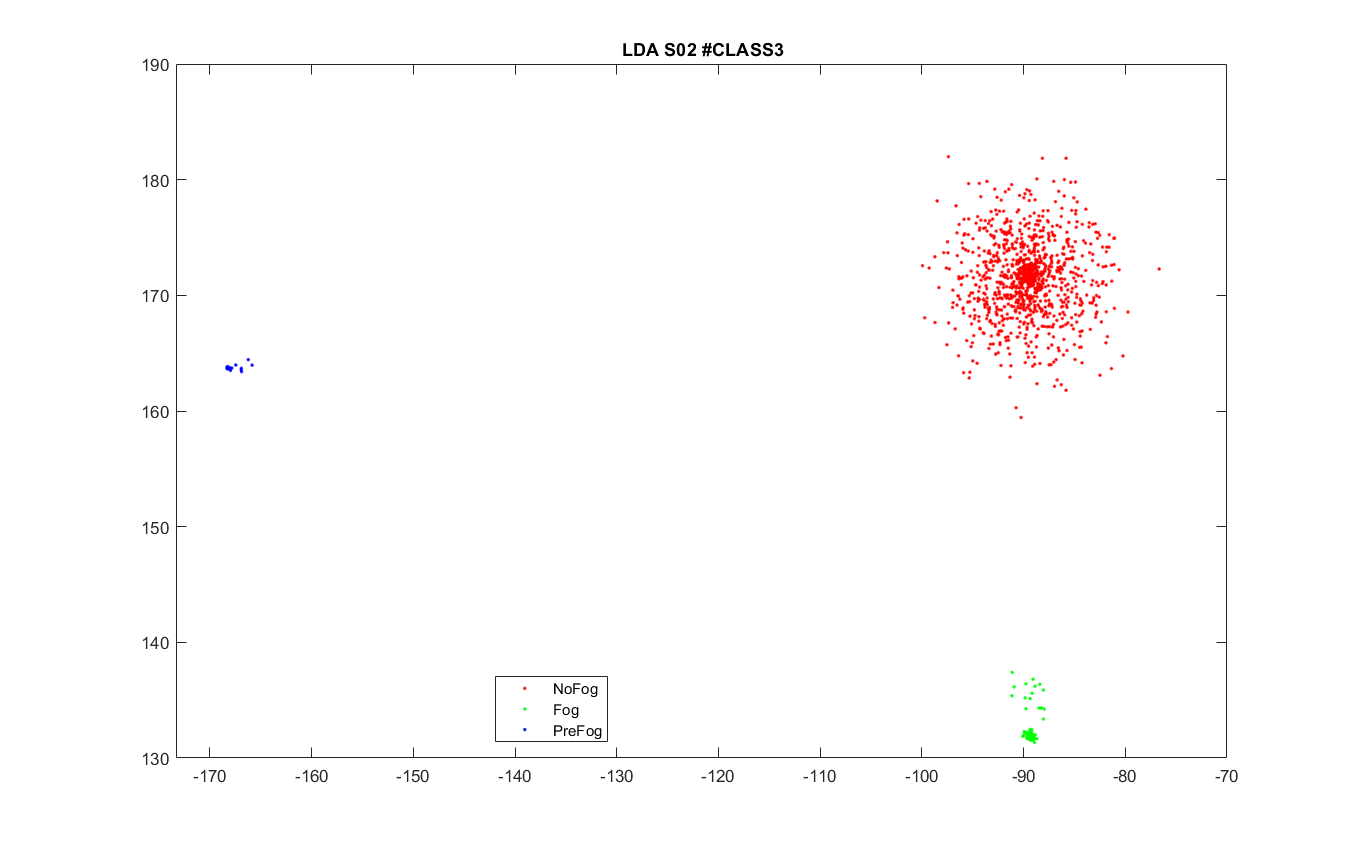
\includegraphics[scale=0.3]{images/LDAS02_best.png}
	\caption{Grafico delle 3 classi in base alla discriminazione dell'approccio di Fisher per il paziente 2 con 2 secondi di finestra ed 1 secondo di overlap}
	\label{LDAS02_best.png}
\end{figure}
\begin{figure}[]
	\centering
	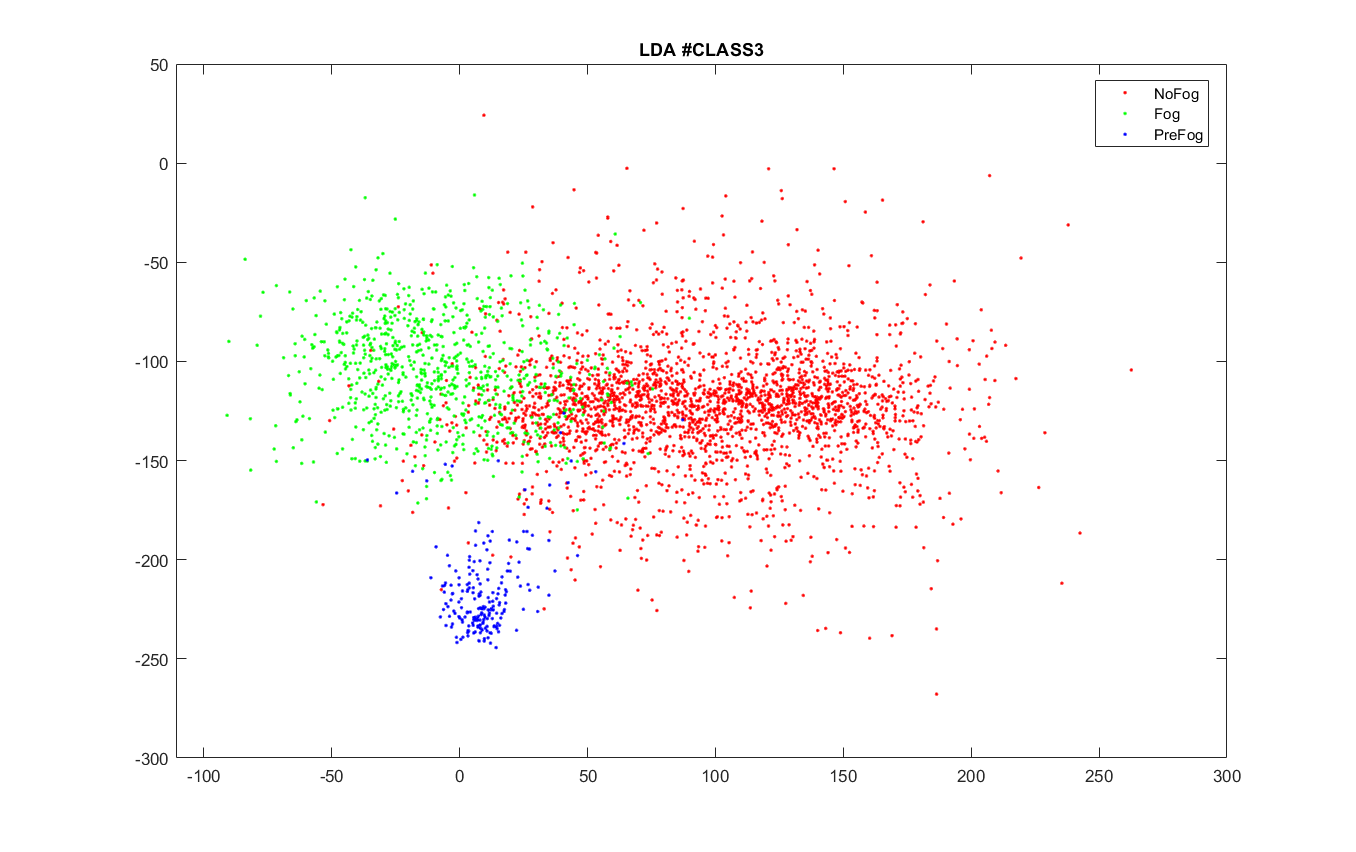
\includegraphics[scale=0.3]{images/LDAALL2.png}
	\caption{Grafico delle 3 classi in base alla discriminazione dell'approccio di Fisher per tutti i pazienti con 2 secondi di finestra ed 1 secondo di overlap}
	\label{LDAALL2.png}
\end{figure}

Dalle tabelle, si nota come il valore di overlap e dimensione della finestra che più frequentemente mi portano ad avere metriche migliori sono:
\begin{itemize}
	\item 1 secondo di sovrapposizione e 2 secondi di finestra;
	\item 1 secondo di sovrapposizione e 1,5 secondi di finestra.
\end{itemize}
L'obiettivo di sostituire il dottore nella prima fase di test, ossia raccogliere dati dagli accelerometri ed applicare le etichette di noFoG, FoG o preFOG, sembra fattibile, in quanto in molti casi abbiamo un'accuratezza vicina al 90\% o comunque superiore al 70\%, per cui la maggior parte delle volte il clustering segna l'etichetta come corretta. Un fatto interessante da notare è che nel caso di pazienti che non hanno avuto episodi di FoG, come il 4 ed il 10, l'accuratezza sia del 100\%, suggerendoci che i movimenti di camminata normale siano comunque diversi da quelli di FoG o preFOG e quindi vengono riconosciuti come tutti simili in assenza di Freezing.\\
Il nostro studio degli intervalli, sia per la parte di clustering che per la parte di LDA, ci porta a concludere che il miglior modo con cui si possono dividere i dati in finestre per calcolare le feature é quello di scegliere 1 secondo per la sovrapposizione tra le finestre ed 1,5 o 2 secondi per quanto riguarda la lunghezza della finestra temporale.

\subsection{Risultati sul singolo paziente}
Per ogni paziente su cui è stata effettuata la prova, abbiamo ricavato la media delle matrici di confusione della cross-validation. Successivamente, prendendo un altro dataset dello stesso paziente, utilizzando il knn allenato abbiamo cercato di predirre le classi del secondo dataset. Poiché non tutti i pazienti presentano, nel dataset, due diversi file (ossia due prove di camminata), la prova è stata possibile solo su alcuni di essi.\\
In tabella \ref{MCcross1} possiamo osservare le matrici di confusione della cross-validation a 10 gruppi per i pazienti numero 1, 2, 3, 5, 7, ossia quelli con doppio file. Si può notare come la matrice risulti diagonali, il che vuole dire che etichetta, nella cross-validation, sempre giusti i nostri campioni sullo stesso paziente.\\
In tabella \ref{MCprev1}, ossia quella relativa alla predizione su un nuovo file, osserviamo che la matrice è abbastanza più confusa, per cui alcune volte etichetta occorrenze di preFOG come altro e non casi di preFOG come preFOG. In tabella \ref{Mpred} si possono osservare le metriche di accuracy, sensitivity, specificity ed F1-measure per la predizione.\\
Questo risultato può essere dato dal fatto che, anche per lo stesso paziente, percorsi diversi o situazioni diverse portano ad una camminata differente da quelle precedenti, e quindi ho dati che possono risultare molto simili ma appartenere a casi diversi nei due test. La cross-validation restituisce delle metriche perfette, quindi l'algoritmo riesce a classificare molto bene i punti di un dataset anche allenandosi solo su una parte di esso e prevedendo i dati esclusi.\\
Il caso della previsione su dati di file diversi, invece, è  da migliorare, in quanto restituisce una specificità bassa, ossia tende a confondere preFOG in NoFoG o FoG. Questo fatto può essere dovuto al fatto che i movimenti, e quindi i dati, di preFOG sono altamente soggettivi e dipendenti dalla situazione in cui il paziente si trova, quindi un movimento nuovo può essere classificato male rispetto al dataset di training. Una possibile soluzione a questo problema sarebbe quello di ottenere dei dataset più grandi, in modo tale da avere un maggior numero di movimenti su cui allenare il classificatore.
% Please add the following required packages to your document preamble:
% \usepackage{multirow}
% \usepackage{graphicx}
\begin{table}[]
	\centering
	\caption{Matrici di confusione per la cross-validation del singolo paziente}
	\label{MCcross1}
	\resizebox{\textwidth}{!}{%
		\begin{tabular}{|c|l|c|c|c|c|c|c|c|c|c|c|}
			\hline
			\textbf{Paziente}                                                                       &                & \textbf{01}                       & \textbf{}                        & \multicolumn{2}{c|}{\textbf{02}}                                     & \multicolumn{2}{c|}{\textbf{03}}                                     & \multicolumn{2}{c|}{\textbf{05}}                                     & \multicolumn{2}{c|}{\textbf{07}}                                     \\ \hline
			\multicolumn{1}{|l|}{}                                                                  & \textbf{Label} & \multicolumn{1}{l|}{\textbf{NPF}} & \multicolumn{1}{l|}{\textbf{PF}} & \multicolumn{1}{l|}{\textbf{NPF}} & \multicolumn{1}{l|}{\textbf{PF}} & \multicolumn{1}{l|}{\textbf{NPF}} & \multicolumn{1}{l|}{\textbf{PF}} & \multicolumn{1}{l|}{\textbf{NPF}} & \multicolumn{1}{l|}{\textbf{PF}} & \multicolumn{1}{l|}{\textbf{NPF}} & \multicolumn{1}{l|}{\textbf{PF}} \\ \hline
			\multirow{2}{*}{\textbf{\begin{tabular}[c]{@{}c@{}}Matrice \\ Confusione\end{tabular}}} & \textbf{NPF}   & 1413                              & 0                                & 431                               & 0                                & 1335                              & 0                                & 983                               & 0                                & 1127                              & 0                                \\ \cline{2-12} 
			& \textbf{PF}    & 0                                 & 36                               & 0                                 & 18                               & 0                                 & 84                               & 0                                 & 76                               & 0                                 & 32                               \\ \hline
		\end{tabular}%
	}
\end{table}
% Please add the following required packages to your document preamble:
% \usepackage{multirow}
% \usepackage{graphicx}
\begin{table}[]
	\centering
	\caption{Matrici di confusione per la previsione del singolo paziente}
	\label{MCprev1}
	\resizebox{\textwidth}{!}{%
		\begin{tabular}{|c|l|c|c|c|c|c|c|c|c|c|c|}
			\hline
			\textbf{Paziente}                                                                       &                & \textbf{01}                       & \textbf{}                        & \multicolumn{2}{c|}{\textbf{02}}                                     & \multicolumn{2}{c|}{\textbf{03}}                                     & \multicolumn{2}{c|}{\textbf{05}}                                     & \multicolumn{2}{c|}{\textbf{07}}                                     \\ \hline
			\multicolumn{1}{|l|}{}                                                                  & \textbf{Label} & \multicolumn{1}{l|}{\textbf{NPF}} & \multicolumn{1}{l|}{\textbf{PF}} & \multicolumn{1}{l|}{\textbf{NPF}} & \multicolumn{1}{l|}{\textbf{PF}} & \multicolumn{1}{l|}{\textbf{NPF}} & \multicolumn{1}{l|}{\textbf{PF}} & \multicolumn{1}{l|}{\textbf{NPF}} & \multicolumn{1}{l|}{\textbf{PF}} & \multicolumn{1}{l|}{\textbf{NPF}} & \multicolumn{1}{l|}{\textbf{PF}} \\ \hline
			\multirow{2}{*}{\textbf{\begin{tabular}[c]{@{}c@{}}Matrice \\ Confusione\end{tabular}}} & \textbf{NPF}   & 412                               & 27                               & 808                               & 173                              & 229                               & 20                               & 621                               & 354                              & 343                               & 90                               \\ \cline{2-12} 
			& \textbf{PF}    & 9                                 & 1                                & 23                                & 10                               & 9                                 & 1                                & 40                                & 14                               & 11                                & 5                                \\ \hline
		\end{tabular}%
	}
\end{table}

% Please add the following required packages to your document preamble:
% \usepackage{graphicx}
\begin{table}[]
	\centering
	\caption{Metriche di misura della predizione per il singolo paziente}
	\label{Mpred}
	\resizebox{\textwidth}{!}{%
		\begin{tabular}{|c|c|c|c|c|}
			\hline
			\multicolumn{1}{|l|}{\textbf{Paziente}} & \multicolumn{1}{l|}{\textbf{Accuracy}} & \multicolumn{1}{l|}{\textbf{Sensitivity}} & \multicolumn{1}{l|}{\textbf{Specificity}} & \multicolumn{1}{l|}{\textbf{F1-measure}} \\ \hline
			\textbf{S01}                            & 0.9198                                 & 0.9385                                    & 0.1000                                    & 0.9581                                   \\ \hline
			\textbf{S02}                            & 0.8067                                 & 0.8236                                    & 0.3030                                    & 0.8918                                   \\ \hline
			\textbf{S03}                            & 0.8880                                 & 0.9197                                    & 0.1000                                    & 0.9404                                   \\ \hline
			\textbf{S05}                            & 0.6171                                 & 0.6369                                    & 0.2593                                    & 0.7591                                   \\ \hline
			\textbf{S07}                            & 0.7751                                 & 0.7921                                    & 0.3125                                    & 0.8716                                   \\ \hline
		\end{tabular}%
	}
\end{table}

\subsection{Risultati usando i dati di tutti i pazienti}
Andando ad usare i dati provenienti da tutti i pazienti, si può osservare in tabella \ref{MCall}, che rappresenta la media delle matrici di confusione della cross-validation e le metriche di accuracy, sensitivity, specificity e F1-measure, come la matrice di confusione non sia diagonale come nel caso del paziente singolo, in quanto pazienti diversi hanno modi di camminare differenti e quindi porta ad avere dati diversi, i quali possono essere classificati nel modo sbagliato. Le metriche comunque sono molto buone, il che ci porta a supporre che molti movimenti di preFOG sono comuni e quindi si può procedere con un modello futuro di previsione di nuovi dati, magari avendo a disposizione dei dataset più grandi ed un numero maggiore di pazienti.
\begin{table}[]
	\centering
	\caption{Matrice confusione e metriche di misura della cross-validation con i dati di tutti i pazienti}
	\label{MCall}
	\resizebox{\textwidth}{!}{%
		\begin{tabular}{|c|l|c|c|c|c|c|c|}
			\hline
			\multicolumn{1}{|l|}{}                                                                  & \textbf{Label} & \multicolumn{1}{l|}{\textbf{NPF}} & \multicolumn{1}{l|}{\textbf{PF}} & \multicolumn{1}{l|}{\textbf{Accuracy}} & \multicolumn{1}{l|}{\textbf{Sensitivity}} & \multicolumn{1}{l|}{\textbf{Specificity}} & \multicolumn{1}{l|}{\textbf{F1-measure}} \\ \hline
			\multirow{2}{*}{\textbf{\begin{tabular}[c]{@{}c@{}}Matrice \\ Confusione\end{tabular}}} & \textbf{NPF}   & 8426                              & 898                              & 0.90                                   & 0.90                                    & 0.89                                 & 0.95                                     \\ \cline{2-8} 
			& \textbf{PF}    & 39                                & 309                              &                                        &                                         &                                      &                                          \\ \hline
		\end{tabular}%
	}
\end{table}

% !TEX root = ../main.tex

% ---------------------------------------------------------------
% Case Studies
% ---------------------------------------------------------------

\chapter{Case Studies}\label{chap7:CS}

%% !TEX root = ../main.tex

\chapter{Experimental Results}\label{chap8:results}
The proposed methodology has been implemented in a tool that automatically generates the self-adaptive wrapper for connecting a cycle-accurate TLM SystemC target to a generic (not necessarily cycle-accurate) TLM SystemC initiator.
Its effectiveness has been evaluated by generating the self-adaptive wrappers for the IPs reported in Table~\ref{TAB:DESIGN}, whose RTL versions have been retrieved from the Open Core Library. Cycle-accurate TLM SystemC models of the considered IPs have been obtained by using HIFSuite-A2T. 
%abstracting the RTL descriptions as reported in Section~\ref{SEC:F_ABSTRACTION}.

Table~\ref{TAB:DESIGN} reports first information related to the RTL version of the IPs, i.e., the number of assertions defined to describe their cycle-accurate communication protocol ($|A|$), the lines of code ($\#lines$), the number of processes ($\#proc$) and the number of input/output ports ($\#I/O$). Then, it reports the number of fields included in the payload of the cycle accurate TLM target ($\#P^T$), which corresponds to $\#I/O-1$ (only clock is removed), and the number of fields included in the payload of the initiator ($\#P^I$), which is lower that $\#P^T$, since the initiator implements a more abstracted loosely timed protocol, where some ports included in the RTL IPs have been removed.

Table~\ref{TAB:RES} reports the simulation times, in seconds, achieved by stimulating each IP with a testbench that generates a sequence of $10^5$ input stimuli. 
The simulation has been performed by composing the testbench, which represents the initiator, and the IP, which represents the target, in different ways and at different abstraction levels.
Column \textit{RTL-TLM (trans)} shows the worst case, where the RTL version of the IP is connected to a loosely timed TLM testbench by means of an ad hoc transactor. This is the simplest solution to reuse an already existing RTL IP inside a TLM design, when a corresponding TLM version of the IP is not available.
On the contrary, Column \textit{LT-LT (no trans)} shows the ideal case, where both the testbench and the target IP implement a perfectly matching, loosely timed TLM protocol. This happens, generally, when the TLM version of the IP is manually implemented. In this case, pin-accurate ports that implement low-level details of the RTL protocol are not included in the payload, thus  the maximum grade of abstraction is reached. In this case, there is no need of generating the transactor between the testbench and the IP. 
Since, manual implementation of a TLM model is time-consuming and error-prone, the fastest and the most safe solution, when an RTL IP of the target design is available, consists of using tools that automatically abstract the IP towards TLM.
Unfortunately, commercial tools that automatically perform RTL-to-TLM abstraction generate cycle-accurate TLM models, since they are not able to automatically abstract low-level details related to the pin-accurate RTL protocol. In such cases, only a TLM cycle-accurate simulation is possible by directly connecting the abstracted IP with a cycle-accurate initiator, which is represented by Column \textit{CA-CA (no trans)}. However, if the initiator implements a more abstracted protocol than a cycle-accurate one, a wrapper is required to allow its communication with the cycle-accurate abstracted IP. This case is showed in Column \textit{LT-CA  (wrapper)}, where we adopted the self-adaptive wrappers that have been automatically generated according to the proposed methodology .

From Table~\ref{TAB:RES} we first observe that for all the benchmarks, but UART, the mixed RTL-TLM simulation via the transactor is orders of magnitude slower than the other simulation schemas. This confirms that the adoption of the transactor generally slows down the overall simulation at the speed of the RTL models, thus making inconvenient the reuse of RTL IPs through transactors. 
This drawback is not particularly evident for the UART, because its RTL model is a structural (not behavioural) description. In such a case, the automatic abstraction of the UART's functionality, via HIFSuite-A2T, generates a TLM version with a low speed-up with respect to the original RTL model. However, this does not depend on the methodology we propose in \chapterref{chap5:Automatic} and \chapterref{chap6:SW_IMP_MET} for the generation of the wrapper, which is independent form the way we abstract the functionality.
Indeed, the efficiency of our self-adaptive wrapper is confirmed by comparing Columns \textit{LT}-LT, \textit{CA-CA} and \textit{LT-CA} for all the benchmarks. The time required by the mixed LT-CA simulation with the use of our wrapper introduces a small overhead in the simulation in comparison with the  LT-LT simulation, and it is faster than the  CA-CA simulation.
This highlights the efficiency of the overall methodology foreseen in \ref{fig:wrapper-gen}, which combines the use of an automatic procedure for abstracting the IP functionality of an RTL IP towards a cycle-accurate TLM model, and the automatic generation of the proposed self-adaptive wrapper to allow the communication between the cycle-accurate TLM model and more abstracted TLM components.



\begin{figure}[h!]
\centering
%\scriptsize
\begin{tabular}{ l || c |c |c |c ||c| c|| }
\multicolumn{1}{l||}{} & 
\multicolumn{4}{c||}{RTL} & 
\multicolumn{2}{c||}{TLM} \\
%\cline{2-7}
$Design$	&	
$|A|$		&	
$\#lines$	&	
$\#proc$	&
$\#I/O$	&
 $\#P^T$	&	
 $\#P^I$\\
\hline
\hline
AES			&	7		&	1778	&	30 	&	8 	& 	7 	&	5	\\
Camellia	&	12		&	955		&	49	&	12	&	11	&	6	\\
DES56 		&	10		&	1054	&	6	&	10	&	9	&	4	\\
UART		&	9		&	3262	&	60	&	23	&	22	&	20\\
%\hline
\end{tabular}
\vspace{0.1cm}
\caption{Characteristics of benchmarks.}
%\vspace{-0.2cm}
\label{TAB:DESIGN}
\end{figure}

\begin{figure}[h!]
\centering
%\scriptsize
\begin{tabular}{ l || c |c |c |c || }
\multirow{2}{*}{$Design$} &
RTL-TLM &
LT-LT &
CA-CA &
LT-CA					\\
						&
$(trans)$ 			&
$(no~trans)$ 	&
$(no~trans)$ 	&
$(wrapper)$				\\
\hline
\hline
AES			&	26495	&844		&904	&			911	\\
Camellia	&	7883	&9			&11		&			10	\\
DES56 		&	410		&45			&54		&			52	\\
UART		&	4300	&3770		&3960	&			3870\\
%\hline
\end{tabular}
\vspace{0.1cm}
\caption{Simulation times (in seconds).}
\vspace{-0.3cm}
\label{TAB:RES}
\end{figure}

% !TEX root = ../main.tex

\chapter{Conclusione e Lavori Futuri}\label{chap9:Concl}
Questa tesi ha proposto una metodologia al fine di verificare l'esistenza di una nuova classe ipotizzata in altri lavori, chiamata preFoG, che si pone come fase di transizione tra un attività normale ed un episodio di Freezing. Riconoscere questa nuova classe permette lo sviluppo di una procedura di previsione del FoG, al fine di far verificare meno episodi possibili di Freezing. Un primo studio dei dati attraverso l'uso di un discriminante lineare ci ha permesso di mostrare e quindi verificare l'effettiva esistenza di questa classe, anche se con una certa sovrapposizione con le altre classi già presenti, dato che al suo interno può contenere movimenti simili a quelli presenti nelle altre classi.\\ 
Per trovare la migliore divisione tra le varie classi, é stato condotto uno studio sulle tempistiche temporali, in cui si é cercato di capire quale fosse la migliore scelta di durata della finestra di divisione dei dati e con quale sovrapposizione. Lo studio é stato condotto sia tramite LDA che con degli approcci di clustering. Questi sono stati usati in quanto permettono un apprendimento non supervisionato dei dati, e quindi l'uso di tali procedimenti potrebbe sostituire il lavoro di etichettatura del medico stesso. Tale studio ci ha portati a definire una finestra di 2 secondi con overlap di 1 secondo come durata migliore degli intervalli temporali al fine di dividere le varie classi. Per la fase non supervisionata di etichettatura dei dati al fine di sostituire il medico, si é arrivati ad un'accuratezza massima del 91\%, con una media, tra i vari pazienti, intorno al 75\%, anche se si hanno ancora dei valori non ottimali per quanto riguarda precisione e recall. Per quei pazienti che non hanno presentato episodi di FoG, comunque, gli algoritmi sono riusciti ad evidenziare tale fatto, il che ci porta a rinforzare l'idea che i movimenti di camminata normale siano differenti sia da quelli di preFoG che di FoG.\\
L'intervallo migliore poi é stato usato per sviluppare un approccio di classificazione tramite LDA, al fine di etichettare nuovi dati. Questo é stato applicato sia su singoli pazienti che su tutti i dati di un test del dataset, al fine di verificare se i movimenti del preFoG fossero simili tra i vari pazienti. Per fare questo, sono state unite le classi di noFOG e FoG, mentre é stata tenuta separata quella di preFoG. Attraverso un processo di cross-validation sui singoli pazienti, questo ci ha portato ad un'accuratezza del 100\%, quindi un riconoscimento perfetto delle occorrenze all'interno dello stesso percorso del paziente. Sui dati di tutti i pazienti, invece, la cross-validation ci ha portati ad un'accuratezza del 90\% e valori simili anche per quanto riguarda la sensitività, specificità e F1-measure, dando ulteriore conferma che i movimenti di preFoG sono più o meno simili anche tra pazienti diversi, almeno all'interno di uno stesso percorso. Questo risultato migliora quanto fatto in \cite{12}, dove attraverso lo stesso test raggiungevano una misura di F1-measure del 70\%.\\
Per quanto riguarda la predizione su nuovi dati, invece, c'é sicuramente ancora lavoro da fare, in quanto i primi test ci hanno portato ad un'alta sensitività ma ad una bassa specificità, il che vuol dire che il classificatore tende a confondere i preFoG quando al paziente si danno da seguire percorsi differenti.
\section{Lavori Futuri}
Tra i possibili lavori futuri c'é sicuramente da continuare sulla classificazione di nuovi dati, andando a migliore quanto più possibile specialmente la specificità della previsione. Questo potrebbe essere svolto anche analizzando algoritmi di classificazione differenti dal knn, magari più complessi ed in grado di catturare in maniera migliore le similarità e le divisioni tra le varie classi.\\
Un ulteriore futuro lavoro é quello di creare una diversa metodologia di estrazione delle feature per quanto riguarda la procedura di clustering e quindi il tentativo di sostituzione del medico nella prima fase di test. Questo può essere fatto, per esempio, scegliendo nuove feature da calcolare.\\
Un ulteriore lavoro futuro, e sicuramente il più interessante ed utile, é quello di applicare tali algoritmi di classificazione e clustering in dispositivi indossabili nella vita quotidiana dal paziente. Questo permetterebbe un riconoscimento real-time delle occorrenze di preFoG per evitare i Freezing e quindi permettere al paziente di bloccarsi il meno possibile. Un ipotetico schema di lavoro é quello presentato in \ref{LavoroFuturo}.
\begin{figure}[h]
	\centering
	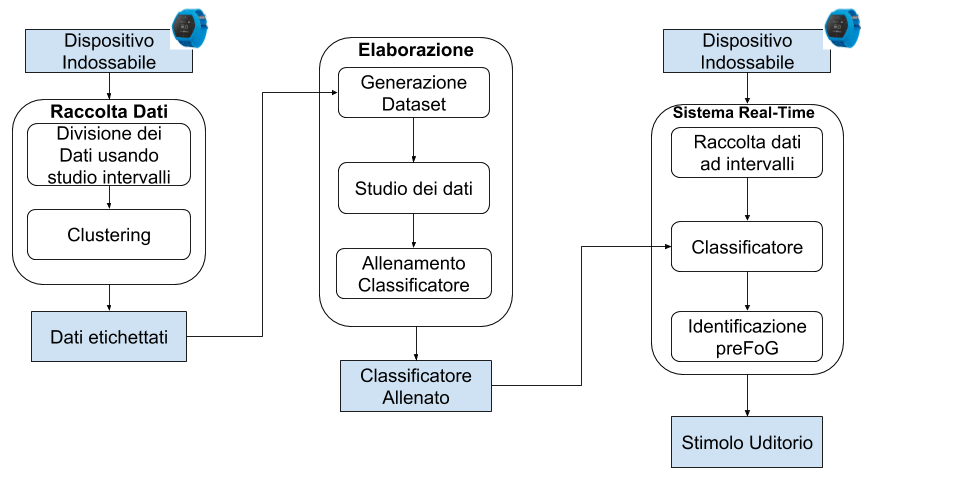
\includegraphics[width=1\textwidth]{images/LavoroFuturo.png}
	\caption{Possibile schema di sistema real-time per l'identificazione del preFoG}
	\label{LavoroFuturo}
\end{figure}


\begin{comment}
% Appendices
\appendix
\setChapters{Appendix}
\renewcommand{\chaptermark}[1]%
{\markboth{\textbf{\appendixname\ \thechapter.\ #1}}{}}
\fancyhead[LO, RE]{\leftmark}
\input{appendices/appendix1.tex}
\end{comment}
% ---------------------------------------------------------------
% Backmatter 
% ---------------------------------------------------------------
\backmatter

% Bibliography
\renewcommand{\chaptermark}[1]%
{\markboth{\textbf{#1}}{}}
\fancyhead[LO, RE]{\leftmark}
\chapter{Bibliography}
%\printbibliography[heading=subbibliography, title={Book References}, filter=books]
%\printbibliography[heading=subbibliography, title={Article References}, filter=papers]
%\printbibliography[heading=subbibliography, title={Other References}, filter=others]
\printbibliography[heading=subbibliography]
% List of acronyms
\chapter*{Acronyms}
\begin{acronym}[AAAAAAAAA]%Longest
\acro{FI}{Freezing Index}
\acro{MEMS}{MicroElectroMechanical Systems}
\acro{PSD}{Power Spectral Density}
\acro{FB}{Freezing Band}
\acro{WB}{Walking Band}
\acro{EMG}{elettromiografia}
\acro{EEG}{elettroencefalogramma}
\acro{FTH}{Freezing Threshold}
\acro{FP}{falsi positivi}
\acro{PI}{Power Index}
\acro{PT}{Power Threshold}
\end{acronym}

\end{document}